% Unified lychee manuscript — compile with xelatex
\documentclass[11pt]{article}

\usepackage[margin=1in]{geometry}
\usepackage{fontspec}
\setmainfont{Times New Roman}
\usepackage{graphicx}
\usepackage{booktabs}
\usepackage{array}
\usepackage{caption}
\usepackage{setspace}
\usepackage[hidelinks]{hyperref}
\usepackage{enumitem}
\usepackage{microtype}

\captionsetup{font=small,labelfont=bf,width=0.94\textwidth}
\setlength{\parskip}{0.35em}
\setlength{\parindent}{1.2em}
\emergencystretch=1.5em
\graphicspath{{figures/}{../../../results/figures/}}

\newcommand{\Pl}{\textit{P.~litchii}}
\newcommand{\q}{\textit{q}}

\title{\bfseries Cultivar-dependent transcriptional responses of lychee (\textit{Litchi chinensis}) to \textit{Peronophythora litchii}: from exploratory candidate discovery to a prospectively registered genome-wide analysis with cross-context external evaluation}
\author{Eric Zhuang}
\date{}

\begin{document}
\maketitle

\begin{abstract}
\noindent
Litchi downy blight, caused by the oomycete \textit{Peronophythora litchii}, is among the most damaging diseases of lychee (\textit{Litchi chinensis} Sonn.), and public RNA-seq cohorts spanning cultivars, tissues, and infection time points offer a natural resource for identifying cultivar-dependent infection responses. Such data are easily over-interpreted, however, when the same cohort is used both to select candidates and to appear to confirm them. Here we unify two stages of a transcriptomic reanalysis of the lychee--\Pl{} interaction into a single account. In the first, exploratory stage, we reanalyzed leaf RNA-seq data from the cultivars Guiwei and Yurong1 (GSE201243/PRJNA830488), identified 17 and 117 infection-responsive genes in the two cultivars, and prioritized 18 candidates with defense-associated annotations and apparently enriched stress- and hormone-associated promoter elements. In the second, confirmatory stage, we prospectively registered a discovery and external-evaluation protocol that fixed dataset roles, statistical models, thresholds, and evidence vocabulary before any external outcome was examined. A genome-wide negative-binomial cultivar-by-infection interaction analysis of 19,445 expressed genes produced 262 statistical candidates, of which 206 were retained after uniform mapping and gene-model quality control, 19 remained significant under an independent genome-wide edgeR quasi-likelihood analysis, and 16 passed the complete registered robustness procedure. In the prespecified cross-context evaluation against an independent pericarp time course contrasting a susceptible and a resistant cultivar (PRJNA450886), two genes were supported and five were directionally contradictory; the internally robust and externally supported sets did not overlap, an outcome compatible with chance given the set sizes. A formal audit showed that none of the original 18 exploratory candidates met the newly applied genome-wide interaction criterion and that two failed uniform-mappability control. Deterministic evidence integration assigned no gene to the highest confidence tier, placed 12 internally robust genes, whose annotations include carbohydrate and cell-wall remodeling, lipid-transfer, and chaperone-regulatory functions, in a middle tier, and retired 65 entities, with all null and contradictory outcomes reported. The unified analysis shows that candidates selected for effect-size prominence in a single cohort largely fail a formally specified genome-wide interaction test, delimits exactly which computational claims about this pathosystem the current public data can support, and releases a candidate resource whose evidence boundaries are explicit. Experimental perturbation remains necessary for any causal conclusion.

\vspace{0.6em}
\noindent\textbf{Keywords:} \textit{Litchi chinensis}; \textit{Peronophythora litchii}; downy blight; RNA-seq; cultivar-by-infection interaction; preregistered analysis; cross-context evaluation
\end{abstract}

\section{Introduction}

Lychee (\textit{Litchi chinensis} Sonn.) is a subtropical fruit crop of substantial economic importance in southern China, Southeast Asia, and a growing set of production regions worldwide [1]. Among its diseases, litchi downy blight, caused by the oomycete \textit{Peronophythora litchii} (historically also treated as \textit{Phytophthora litchii} [2]), is particularly damaging: the pathogen attacks young leaves, inflorescences, and fruit, produces water-soaked brown lesions, and drives severe postharvest decay [2,3]. Because chemical control is costly and resistance breeding depends on understanding how host genotypes differ in their response to infection, the molecular basis of cultivar-level variation in the response to \Pl{} is a question of both agronomic and biological interest.

The resources needed to address this question computationally have accumulated rapidly. High-quality genome assemblies are available for lychee [4], and several groups have profiled the transcriptional response to \Pl{} infection. Sun et al.\ compared a susceptible and a resistant cultivar across a pericarp infection time course and reported that the two genotypes deploy distinct early response programs [5]. Liu et al.\ described calcium-dependent protein kinase (LcCDPK) family members induced by \Pl{} inoculation [6], and Li et al.\ showed that the pathogen RXLR effector PlAvh202 promotes virulence by destabilizing a host ethylene-biosynthesis enzyme [7]. A pathogen-side transcriptome catalogued the \Pl{} pathogenicity arsenal [2]. In parallel, public repositories now hold RNA-seq series covering resistant and susceptible cultivars, leaf and fruit tissues, messenger and small RNA, and multiple time points. These series offer an opportunity, in principle, to distinguish genome-wide cultivar-dependent infection responses from responses common to all genotypes.

Realizing that opportunity is statistically demanding. The quantity of interest is not differential expression within a cultivar but the cultivar-by-infection interaction: the difference between infection responses across genotypes. Interaction effects are estimated with less precision than main effects, the deposited designs are small (typically three libraries per cultivar--treatment cell), and a genome-wide search requires an explicit multiplicity family. Analyses that instead select a handful of strongly responding genes and then characterize them in the same cohort conflate selection with confirmation: large observed fold changes in a small experiment are a mixture of true signal and noise, and features chosen for extremity will regress toward null in any independent assessment. These concerns apply directly to the present pathosystem, in which most published candidate genes derive from single-cohort analyses without external evaluation.

The first stage of the present work followed the same pattern. In an exploratory reanalysis of the GSE201243 leaf series [8] (Guiwei and Yurong1, mock versus inoculated, 24~h post-inoculation), we identified 17 significant infection-responsive genes in Guiwei and 117 in Yurong1, prioritized 18 candidates with defense-plausible annotations (among them jacalin-like lectin, pathogenesis-related and thaumatin/osmotin-like proteins, a heat-shock protein, lipid-transfer proteins, and calcium-binding proteins), and found that a set of stress- and hormone-associated \textit{cis}-regulatory elements was enriched in their promoters relative to a randomized background. That analysis was framed as hypothesis-generating, and critical review of it converged on three substantive criticisms: the cultivar-by-treatment comparison was an effect-size contrast over pre-selected genes rather than a genome-wide interaction test with false-discovery-rate control; no independent dataset was used for validation; and promoter-element counting, even against a randomized background, is weak evidence of regulatory function. We regard all three criticisms as correct, and they motivated the confirmatory stage reported here.

This paper therefore presents the complete arc of the project in one place. We prospectively registered a discovery and external-evaluation protocol that fixed dataset roles, models, thresholds, empty-result behavior, and the vocabulary used to describe evidence before any external outcome was opened. Because every cohort is public, this staged unlock is a computational safeguard enforced by the workflow rather than blinding in the experimental sense, and we document the registration chronology in the Methods. Within the prespecified discovery cohort we fitted a genome-wide negative-binomial interaction model, applied uniform mapping and gene-model quality control, and subjected the resulting candidates to a battery of internal robustness checks spanning independent quantification, an alternative statistical framework, filter sensitivity, and leave-one-library-out refits. We then evaluated the frozen candidates (throughout, \emph{frozen} denotes a computed result fixed at a recorded checkpoint and not modified afterward), a frozen pathway set, and a frozen signed expression signature in independent public cohorts whose roles (primary cross-context evaluation, generic transfer, orthogonal modality, or exploratory) were fixed in advance. Orthogonal evidence classes (sequence annotation, promoter motifs, small-RNA coherence, and accession-aware literature) were kept separate from expression support, and a deterministic tier system integrated all layers while explicitly permitting an empty top tier. Finally, we audited the 18 exploratory candidates from the first stage against the genome-wide analysis. The result is a candidate resource for lychee downy blight whose every claim carries its evidence class, together with a case study in how much, and how little, of a plausible exploratory analysis survives formal statistical scrutiny.

\section{Results}

\subsection{A two-stage design with prespecified dataset roles}

The study comprises an exploratory stage completed first and a confirmatory stage whose protocol was registered before its analyses began (Figure~\ref{fig:design}A; Table~\ref{tab:roles}). Five public cohorts enter the confirmatory stage in fixed, non-interchangeable roles. PRJNA830488 (GSE201243), the leaf series for Guiwei and Yurong1 at 24~h, is the sole discovery cohort; it is also the dataset analyzed in the exploratory stage. PRJNA450886, a pericarp time course contrasting the susceptible cultivar Guiwei with the resistant cultivar Heiye at 6, 24, and 48~h [5], serves as the primary external evaluation. Because it differs from the discovery cohort in tissue, resistant comparator, and time structure, we describe positive outcomes in it as \emph{cross-context support} rather than replication. PRJNA922966 (Feizixiao leaf and fruit, mock versus infected) tests generic infection-response transfer but cannot address the cultivar interaction; PRJNA922965 provides small-RNA libraries as an orthogonal modality; and PRJNA1090613 (Guiwei versus SFZ leaf) is exploratory only, because its time and resistance metadata could not be resolved. Under the registered firewall, no external outcome could alter the frozen discovery membership, signature weights, or thresholds, and the protocol explicitly allowed the top evidence tier to be empty.

\begin{figure}[p]
\centering
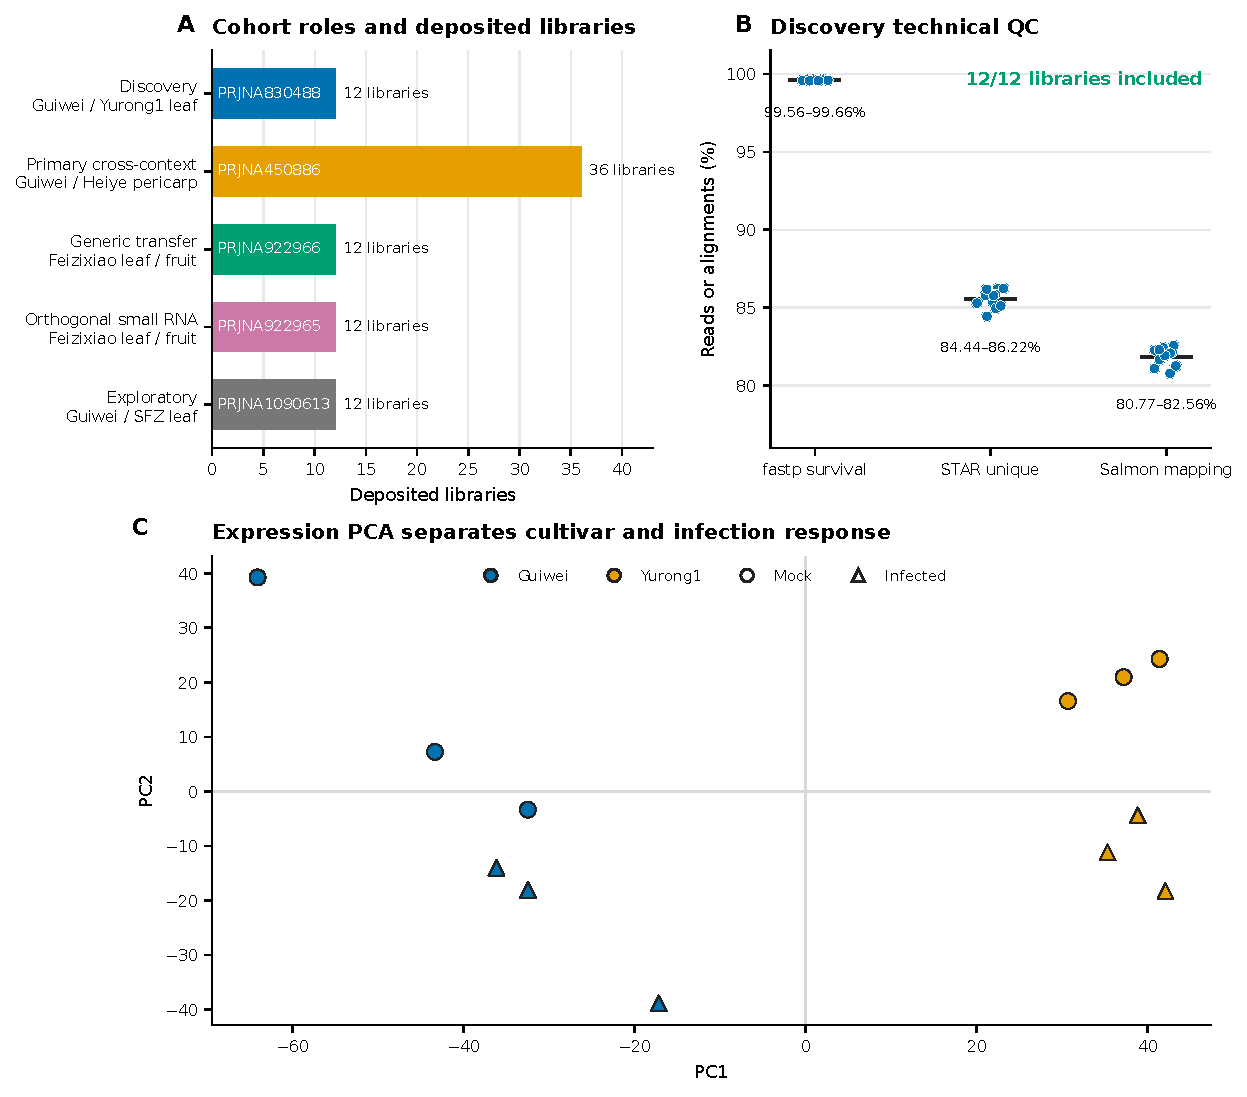
\includegraphics[width=0.98\textwidth]{figure1_study_design_qc.pdf}
\caption{\textbf{Study cohorts, discovery quality control, and expression structure.} (A) The five public cohorts with prespecified roles and deposited library counts. (B) Per-library technical quality in the discovery cohort: fastp read survival, STAR unique-alignment rate, and Salmon mapping rate; all 12 libraries passed the fixed inclusion gates. (C) Principal-component analysis of the discovery libraries separates cultivar and infection status.}
\label{fig:design}
\end{figure}

\begin{table}[t]
\centering
\caption{\textbf{Locked dataset roles and eligibility.}}
\label{tab:roles}
\small
\begin{tabular}{@{}p{3.2cm}p{5.6cm}p{3.3cm}p{2.6cm}@{}}
\toprule
\textbf{Accession} & \textbf{Design} & \textbf{Locked role} & \textbf{Evidence class} \\
\midrule
PRJNA830488 (GSE201243) & Guiwei/Yurong1 leaf; mock/infected; 24 h; 3 libraries per cell & Discovery & Conditional inferential \\
PRJNA450886 & Guiwei/Heiye pericarp; mock/infected; 6, 24, 48 h; 3 libraries per cell & Primary external evaluation & Cross-context \\
PRJNA922966 (GSE222651) & Feizixiao leaf/fruit; mock/infected; 24 h; 3 libraries per cell & Generic infection transfer & Cross-context \\
PRJNA922965 (GSE222650) & Feizixiao leaf/fruit small RNA; mock/infected; 24 h; 3 libraries per cell & Orthogonal modality & Orthogonal \\
PRJNA1090613 (GSE262200) & Guiwei/SFZ leaf; mock/infected; 3 libraries per cell & Exploratory only & Exploratory \\
\bottomrule
\end{tabular}
\end{table}

\subsection{Stage 1: exploratory candidate discovery in GSE201243}

The exploratory stage analyzed the 12 discovery libraries with per-cultivar differential-expression contrasts (infected versus mock) and identified 17 significant genes in Guiwei (15 up-regulated, 2 down-regulated) and 117 in Yurong1 (39 up-regulated, 78 down-regulated) at Benjamini--Hochberg adjusted $P<0.05$, suggesting a broader transcriptional response in Yurong1. From these lists, 18 genes were prioritized by combining statistical significance in at least one cultivar, large infection-associated fold changes, and annotations plausibly related to defense: among them a jacalin-like lectin (LITCHI028104), a pathogenesis-related protein (LITCHI011394), osmotin/thaumatin-like proteins (LITCHI009301, LITCHI002793), an HSP70-family chaperone (LITCHI012388), lipid-transfer proteins (LITCHI019183, LITCHI018043), an EF-hand calcium-binding protein (LITCHI019519), and a phytosulfokine precursor (LITCHI007102). A selected-gene contrast of infection responses between cultivars nominated LITCHI019519, LITCHI001510, LITCHI028401, and LITCHI017676 as Guiwei-skewed and LITCHI028104 and LITCHI019183 as Yurong1-skewed candidates.

The exploratory stage also examined 2-kb upstream promoter regions of the 18 candidates. Against 100,000 randomized GC-matched promoter sets, four \textit{cis}-element classes appeared enriched: anaerobic-response elements (ARE; 46 observed versus 24.6 expected, $\q=0.0003$), methyl-jasmonate-responsive motifs (54 versus 38.4, $\q=0.018$), TCA elements (9 versus 0.19, $\q=0.00003$), and TC-rich repeats (10 versus 0.15, $\q=0.00003$). ABRE and MYB-binding-site motifs, in contrast, were frequent but not enriched. All of these results were obtained by selecting and characterizing genes within a single cohort; they carry no genome-wide multiplicity control and no external evaluation, and we treat them below strictly as hypotheses submitted to the confirmatory stage.

\subsection{Discovery-cohort quality under the registered protocol}

The confirmatory pipeline combined a joint host and pathogen reference, fastp trimming, STAR two-pass alignment, featureCounts gene counting, and independent Salmon quantification. Under this pipeline, all 12 discovery libraries passed the fixed technical gates of at least 10 million surviving read pairs and at least 40\% uniquely aligned reads (Figure~\ref{fig:design}B). Read survival after trimming ranged from 99.56\% to 99.66\%, unique-alignment rates from 84.44\% to 86.22\%, and Salmon mapping rates from 80.77\% to 82.56\%. Principal-component analysis of the transformed counts separated libraries by cultivar on the first component (54.2\% of variance) and by infection status on the second (16.1\%), with no library isolated from its replicate group (Figure~\ref{fig:design}C). Because source-tree, pooling, and extraction independence are not reported for the deposited libraries, all inferential statements below are conditional on deposited-library independence, a limitation we return to in the Discussion.

\subsection{Genome-wide cultivar-by-infection discovery}

The primary discovery model fitted all expressed genes with the design $\sim$ cultivar + treatment + cultivar:treatment, with Guiwei and mock as reference levels, so that the interaction coefficient estimates how much the infected-minus-mock response in Yurong1 exceeds that in Guiwei. Of 19,445 expressed genes, 262 met the registered discovery threshold of genome-wide Benjamini--Hochberg $\q<0.05$ with an absolute interaction log2 fold change of at least $\log_2(1.5)$ (Figure~\ref{fig:discovery}A); 277 genes met the significance criterion alone and 5,370 met the effect criterion alone. All interaction estimates reported and plotted here are unshrunken maximum-likelihood values; apeglm shrinkage was used only to define the frozen signature weights. Uniform quality control then removed 31 candidates for exon-level mappability failure and 25 for gene-model ambiguity, freezing 206 genes as statistical candidates (Figure~\ref{fig:discovery}C). Because these quality filters were applied after significance testing, we verified that the ordering is not load-bearing: restricting the testing universe to the 13,602 genes that pass uniform quality control and recomputing the Benjamini--Hochberg adjustment over that universe rediscovers all 206 frozen candidates and adds 12 further genes, so the frozen list is a conservative subset of the QC-first analysis. A post hoc composite-null sensitivity analysis asked the stricter question whether $|\beta|$ exceeded $\log_2(1.5)$, rather than testing $\beta=0$ and filtering the estimate afterward. Eight of the 262 statistical candidates passed the DESeq2 composite-null test at $\q<0.05$; the corresponding counts were 7 of 206 QC-retained candidates, 7 of 19 edgeR-gated candidates, and 7 of 16 fully robust candidates. An apeglm false-sign-or-small analysis was less severe, with $s<0.05$ for 149, 113, 18, and 15 genes in those four nested sets, respectively. These are post hoc sensitivity results, not a redefinition of the registered discovery set. Positive interaction effects (stronger infection response in Yurong1) and negative effects (stronger response in Guiwei) were both well represented. At the pathway level, six Plant Reactome pathways transported through one-to-one \textit{Oryza} orthology met the frozen discovery threshold: activation of the pre-replication complex, assembly of the pre-replication complex, DNA replication initiation, maturation, and circadian rhythm, all with positive enrichment, and jasmonic acid signaling with negative enrichment. Together with the genes, these six pathways, the apeglm-shrunken signed signature weights over the 206 genes, and the conditional transcript-usage results (Section~2.9) were frozen before any external data were opened.

\begin{figure}[p]
\centering
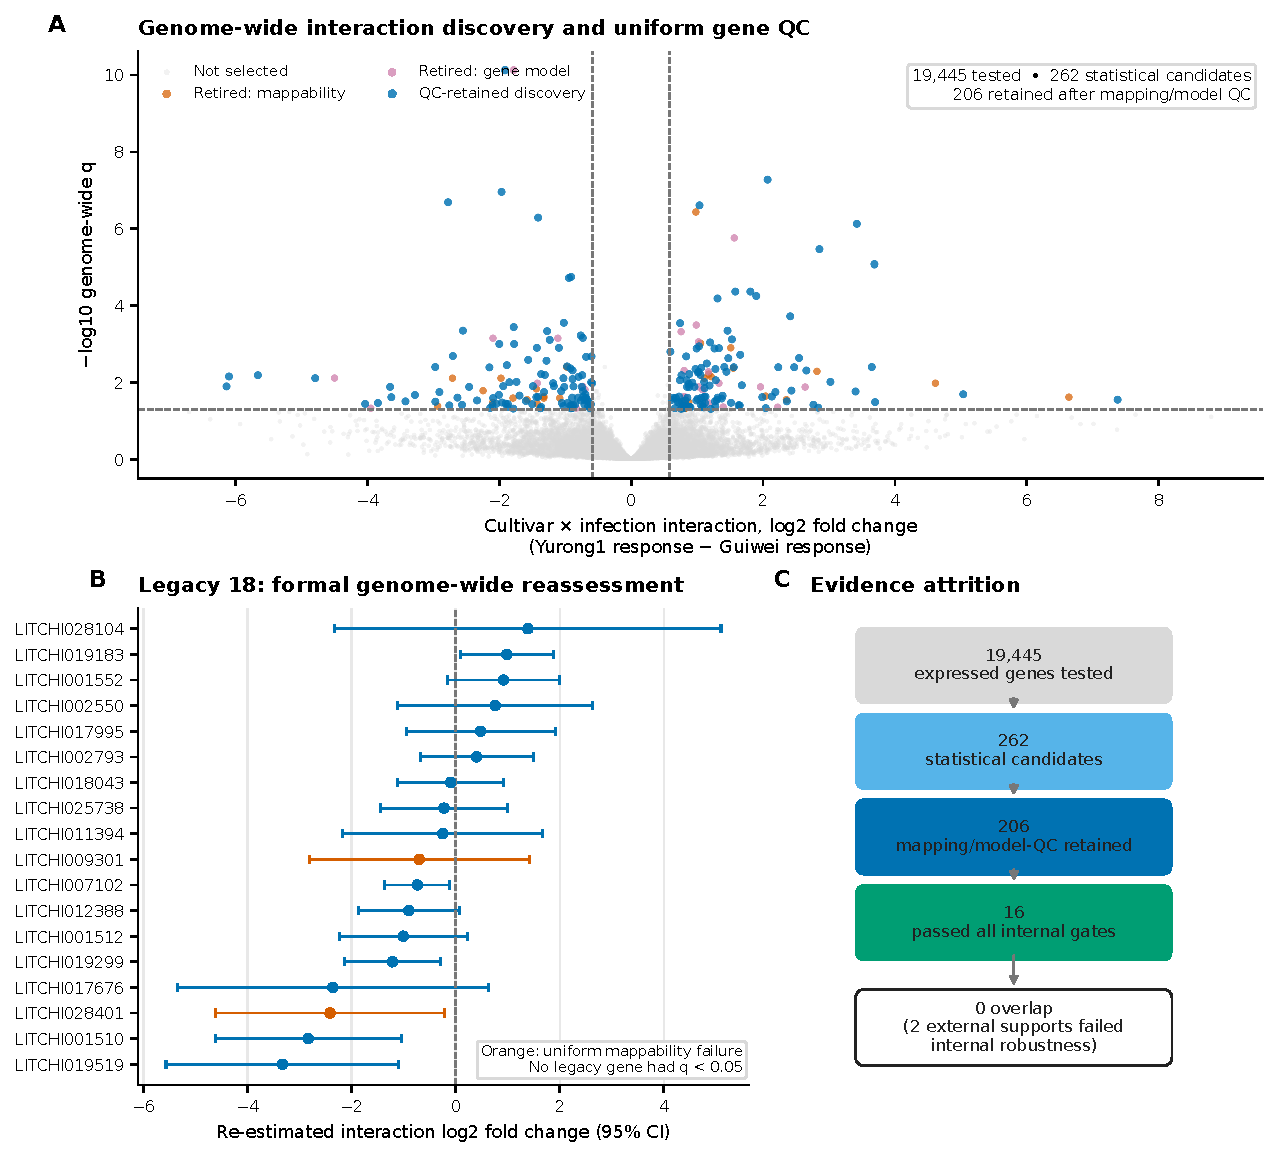
\includegraphics[width=0.98\textwidth]{figure2_discovery_legacy.pdf}
\caption{\textbf{Genome-wide discovery and formal reassessment of the exploratory candidates.} (A) Cultivar-by-infection interaction effects across 19,445 expressed genes; 262 genes met the statistical threshold and 206 were retained after uniform mapping and gene-model quality control. (B) Genome-wide re-estimation of the 18 exploratory (legacy) candidates with 95\% confidence intervals; orange marks uniform-mappability failures. No legacy candidate met the genome-wide interaction criterion. (C) Evidence attrition from tested genes to internally robust candidates.}
\label{fig:discovery}
\end{figure}

\subsection{None of the 18 exploratory candidates met the genome-wide interaction criterion}

Because the exploratory candidates were selected before any interaction $P$-values existed, the registered protocol included a formal audit of all 18 against the genome-wide analysis (Figure~\ref{fig:discovery}B; Table~\ref{tab:legacy}). None met the genome-wide interaction threshold. We then performed the estimand-aligned follow-up requested in review: separate confirmatory DESeq2 infected-versus-mock fits within each cultivar, with Benjamini--Hochberg adjustment over the same 19,445-gene universe in each contrast (Supplementary S14). Thirteen of the 18 legacy genes were significant in Guiwei and 16 of 18 in Yurong1 at $\q<0.05$; all 13 Guiwei genes and 15 of the 16 Yurong1 genes also exceeded $|\mathrm{log2FC}|\ge\log_2(1.5)$. Thus most of the original within-cultivar response claims survive the confirmatory pipeline even though none supports a genome-wide cultivar-by-infection interaction. The strongest interaction-audit candidate, LITCHI001510, reached $\q=0.080$; the EF-hand calcium-binding gene LITCHI019519, whose selected-gene contrast of $-3.4$ had appeared most dramatic in the exploratory stage, reached only $\q=0.106$ despite a re-estimated interaction effect of $-3.33$; and the median genome-wide interaction \q{} across the 18 candidates was 0.47. Two candidates, the osmotin/thaumatin-like gene LITCHI009301 and LITCHI028401, additionally failed uniform exon-mappability control, meaning their interaction estimates cannot be attributed unambiguously to a single locus. The audit therefore does not show that these genes are biologically inert. It shows that within-cultivar responsiveness and cultivar-dependent response are distinct claims, and only the latter fails here.

\begin{table}[p]
\centering
\caption{\textbf{Formal genome-wide audit of the 18 exploratory-stage candidates.} Interaction effects are re-estimated genome-wide values (Yurong1 response minus Guiwei response, log2 scale). No candidate met the registered discovery threshold (genome-wide $\q<0.05$ and $|\mathrm{log2FC}|\ge\log_2(1.5)$).}
\label{tab:legacy}
\footnotesize
\begin{tabular}{@{}llccc@{}}
\toprule
\textbf{Gene} & \textbf{Exploratory annotation} & \textbf{Interaction log2FC (SE)} & \textbf{Genome-wide \q} & \textbf{Mappability} \\
\midrule
LITCHI001510 & Poorly characterized responsive gene & $-2.83$ (0.91) & 0.080 & Pass \\
LITCHI019519 & EF-hand calcium-binding protein & $-3.33$ (1.14) & 0.106 & Pass \\
LITCHI019299 & S-adenosylmethionine-related protein & $-1.21$ (0.47) & 0.175 & Pass \\
LITCHI007102 & Phytosulfokine precursor & $-0.74$ (0.32) & 0.238 & Pass \\
LITCHI019183 & Plant lipid-transfer protein & $+0.99$ (0.45) & 0.273 & Pass \\
LITCHI028401 & Selected interaction candidate & $-2.41$ (1.13) & 0.281 & Fail \\
LITCHI012388 & Heat-shock protein 70 & $-0.90$ (0.49) & 0.381 & Pass \\
LITCHI001552 & Cyclase-like stress-related protein & $+0.92$ (0.55) & 0.430 & Pass \\
LITCHI001512 & Poorly characterized responsive gene & $-1.01$ (0.63) & 0.457 & Pass \\
LITCHI017676 & S-adenosylmethionine-related protein & $-2.36$ (1.53) & 0.478 & Pass \\
LITCHI002550 & Cytochrome P450 & $+0.76$ (0.96) & 0.762 & Pass \\
LITCHI028104 & Jacalin-like lectin & $+1.39$ (1.89) & 0.785 & Pass \\
LITCHI002793 & Osmotin/thaumatin-like protein & $+0.41$ (0.55) & 0.786 & Pass \\
LITCHI017995 & Metalloendoproteinase & $+0.48$ (0.73) & 0.812 & Pass \\
LITCHI009301 & Osmotin/thaumatin-like protein & $-0.70$ (1.08) & 0.816 & Fail \\
LITCHI025738 & Cyclase-like stress-related protein & $-0.22$ (0.62) & 0.908 & Pass \\
LITCHI011394 & Pathogenesis-related protein & $-0.25$ (0.98) & 0.940 & Pass \\
LITCHI018043 & Plant lipid-transfer protein & $-0.10$ (0.52) & 0.954 & Pass \\
\bottomrule
\end{tabular}
\end{table}

\subsection{Sixteen genes and one pathway passed all internal robustness gates}

Each of the 206 frozen genes was required to retain its interaction direction and significance under four predeclared perturbations of the analysis: independent Salmon-based quantification (196 of 206 passed), edgeR quasi-likelihood testing in place of the primary framework (19 passed), a counts-per-million expression filter (205 passed), and all twelve leave-one-library-out refits (125 passed). Eighteen genes passed all four gates jointly, and 16 remained after an additional observed mapping-sensitivity gate that excluded candidates whose effect depended on ambiguously mapped reads (Figure~\ref{fig:robust}A). The alternative-framework gate was by far the most stringent, and the frozen genome-wide edgeR results explain why. The two frameworks agree almost perfectly on estimation: interaction effects correlate at Pearson $r=0.995$ across all 19,445 genes and $r=0.999$ across the 206 candidates, sign agreement among the candidates is 100\%, and every candidate has nominal edgeR $P<0.05$. The disagreement is confined to significance calibration. The registered gate required genome-wide edgeR $\q<0.10$ with direction agreement, and edgeR's quasi-likelihood test with robust dispersion estimation admits only 24 genes genome-wide at that threshold (10 at $\q<0.05$), against 262 for the primary Wald analysis at $\q<0.05$. With three libraries per cell, the two dispersion-estimation strategies imply very different genome-wide significance sets even while agreeing on every point estimate. We therefore present the results as a hierarchy: 262 statistical candidates, 206 retained after quality control, 19 significant under both frameworks, and 16 passing the complete registered procedure; genes surviving both frameworks constitute the discovery set's stable core, and the wider 206-gene list should be read as one framework's candidates rather than as settled discoveries. Of the six frozen pathways, only circadian rhythm passed its four conjunctive gates (competitive and rotation-based testing, leading-edge deletion, and an expression- and length-matched null); the other five all failed the rotation-based self-contained test, and the maturation set additionally failed leading-edge deletion, indicating enrichment that was not stable across testing frameworks.

\begin{figure}[p]
\centering
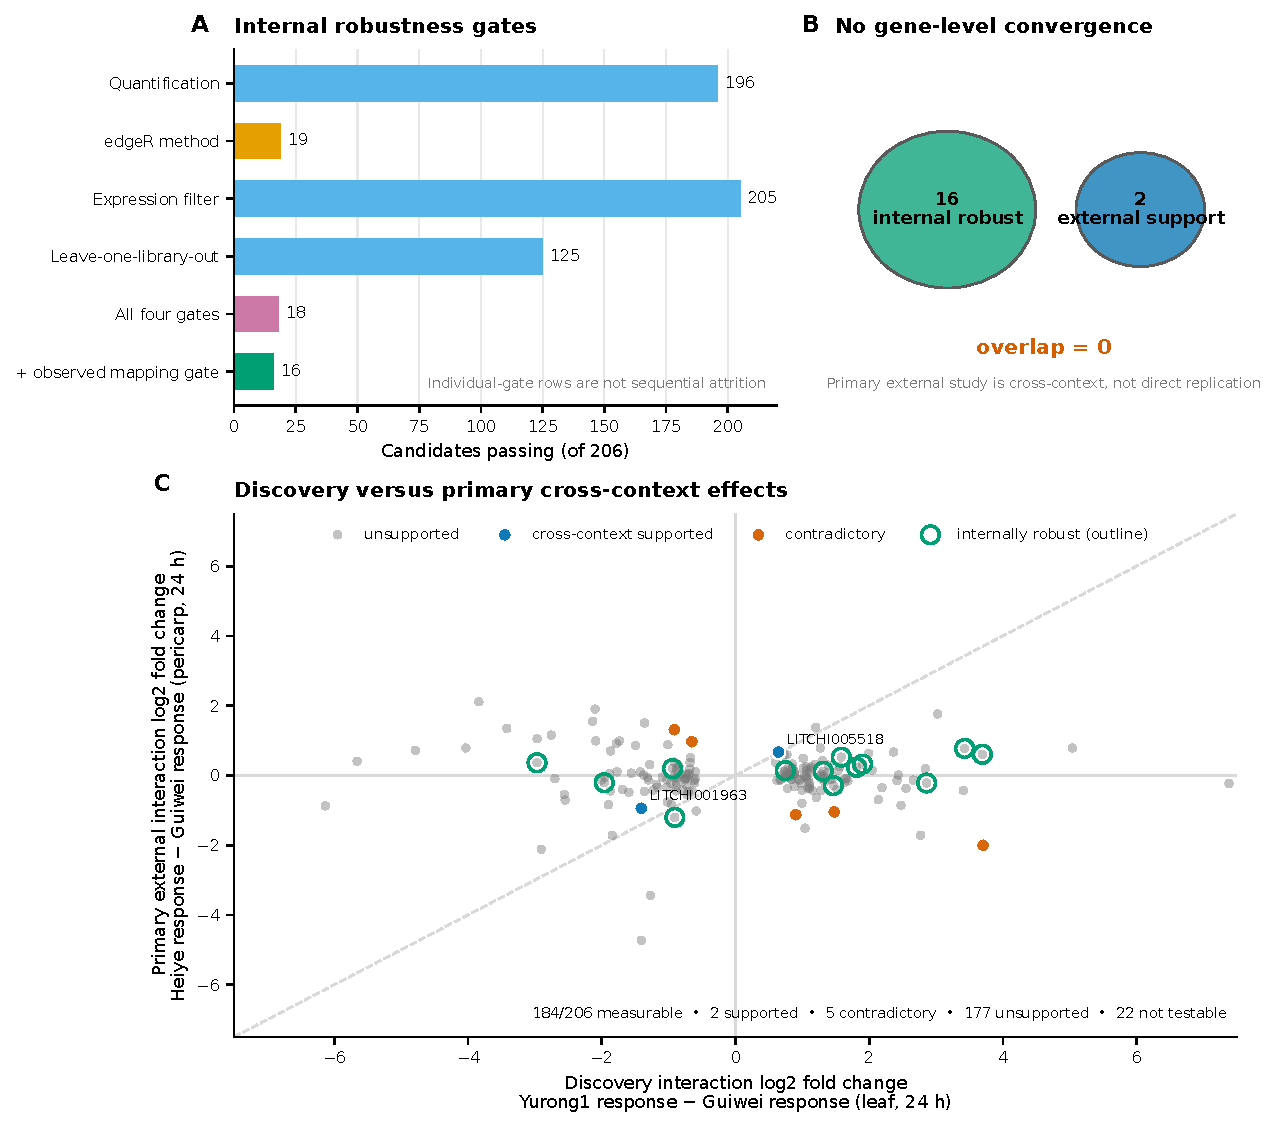
\includegraphics[width=0.98\textwidth]{figure3_robustness_external.pdf}
\caption{\textbf{Internal robustness and the primary external evaluation.} (A) Candidates passing each predeclared robustness gate, the conjunction of the four analytic gates, and the additional observed-mapping gate. (B) The internally robust set (16 genes) and the externally supported set (2 genes) do not overlap. (C) Discovery interaction effects against the primary cross-context interaction effects (Heiye response minus Guiwei response, pericarp, 24 h); supported, contradictory, and internally robust genes are highlighted. The diagonal is a visual reference only; equal effects across contexts are not expected.}
\label{fig:robust}
\end{figure}

\subsection{The prespecified external evaluation supported two genes and contradicted five}

The primary external estimand, fixed before unlock, was the resistant-minus-susceptible cultivar-by-infection interaction at 24~h in the PRJNA450886 pericarp time course, tested for each frozen candidate with Benjamini--Hochberg adjustment across the full candidate-by-contrast family, an effect threshold of $\log_2(1.5)$, confidence intervals excluding zero, and required agreement with the discovery direction. Of the 206 frozen genes, 184 were measurable in the external cohort. Two met every criterion and are cross-context supported: LITCHI005518, annotated as an alpha-xylosidase involved in xyloglucan remodeling of the cell wall, and LITCHI001963, an uncharacterized gene with a one-to-one \textit{Oryza} ortholog. Five genes, including a beta-glucosidase and a Fe(II)/2-oxoglutarate-dependent dioxygenase, passed the magnitude and significance criteria with the \emph{opposite} direction and are recorded as contradictory; 177 were unsupported at the prespecified thresholds and 22 not testable (Figure~\ref{fig:robust}C; Table~\ref{tab:external}). At the level of continuous estimates, discovery and external interaction effects across the 184 measurable candidates were uncorrelated (Pearson $r=-0.05$, 95\% CI $-0.19$ to 0.10; Spearman $\rho=-0.04$), with sign concordance of 51.6\% (95 of 184), indistinguishable from chance.

The two supported genes are not among the 16 internally robust genes, and none of the 16 internally robust genes achieved external support (Figure~\ref{fig:robust}B). This non-overlap is, by itself, nearly uninformative: for sets of 16 and 2 genes drawn from 206 candidates, the expected overlap under independence is 0.16 genes and the probability of zero overlap is 0.85, so the disjoint sets neither demonstrate nor refute an association between internal stability and cross-context transport. The absence of continuous concordance reported above is the more informative observation. We emphasize that the external cohort differs in tissue (pericarp versus leaf), resistant comparator (Heiye versus Yurong1), and design (time course versus single time point), so absence of support is expected wherever a response is tissue- or genotype-specific, and support that is observed indicates transport across contexts rather than replication of the original experiment. Because Yurong1 and Heiye have not been placed on a common resistance scale relative to Guiwei, we interpret the primary external test as cross-cultivar response transport rather than validation of a resistance phenotype.

\begin{table}[p]
\centering
\caption{\textbf{Cross-context supported and contradictory genes in the primary external evaluation (PRJNA450886, pericarp, 24 h).} Discovery effects are Yurong1-minus-Guiwei interaction log2 fold changes in leaf; external effects are Heiye-minus-Guiwei interaction log2 fold changes in pericarp with 95\% confidence intervals. All \q-values are Benjamini--Hochberg adjusted (discovery: genome-wide; external: across the frozen candidate-by-contrast family).}
\label{tab:external}
\footnotesize
\setlength{\tabcolsep}{2.4pt}
\begin{tabular}{@{}llccccc@{}}
\toprule
\textbf{Gene} & \textbf{Annotation} & \textbf{Disc.\ log2FC} & \textbf{Disc.\ \q} & \textbf{Ext.\ log2FC (95\% CI)} & \textbf{Ext.\ \q} & \textbf{Outcome} \\
\midrule
LITCHI005518 & Alpha-xylosidase 1 & $+0.64$ & 0.025 & $+0.67$ ($+0.32$ to $+1.02$) & 0.007 & Supported \\
LITCHI001963 & Uncharacterized; 1:1 \textit{Oryza} ortholog & $-1.41$ & 0.024 & $-0.94$ ($-1.43$ to $-0.46$) & 0.007 & Supported \\
LITCHI030761 & Caffeoylshikimate esterase & $-0.92$ & 0.040 & $+1.31$ ($+0.78$ to $+1.85$) & 0.0002 & Contradictory \\
LITCHI029534 & Thiamine thiazole synthase 2 & $+1.48$ & 0.002 & $-1.04$ ($-1.61$ to $-0.48$) & 0.010 & Contradictory \\
LITCHI021860 & Phosphatidylinositol 4-kinase gamma 2 & $-0.65$ & 0.032 & $+0.97$ ($+0.39$ to $+1.54$) & 0.029 & Contradictory \\
LITCHI008313 & Beta-glucosidase 44 & $+0.90$ & 0.045 & $-1.12$ ($-1.81$ to $-0.44$) & 0.034 & Contradictory \\
LITCHI001700 & Fe(II)/2-OG-dependent dioxygenase 4 & $+3.70$ & 0.033 & $-2.00$ ($-3.24$ to $-0.77$) & 0.035 & Contradictory \\
\bottomrule
\end{tabular}
\end{table}

\subsection{Pathway and signature transport was weak and strongly context-dependent}

None of the six frozen pathways, including the internally robust circadian-rhythm pathway, passed the external pathway gates in PRJNA450886 (Figure~\ref{fig:pathways}A). The frozen signed signature over the 206 discovery genes behaved in a strongly context-dependent way (Figure~\ref{fig:pathways}B). At the primary 24-h contrast the signature score was indistinguishable from zero (estimate 0.109, 95\% CI $-0.079$ to 0.297, $\q=0.349$), and at 48~h it was significantly \emph{negative} ($-0.240$, 95\% CI $-0.428$ to $-0.052$, $\q=0.043$), a sign reversal relative to discovery. In the generic-transfer study the signature tracked infection positively in leaf (0.107, $\q=0.0015$) but negatively in fruit ($-0.181$, $\q<0.001$), with a significant leaf-minus-fruit interaction (0.289, $\q<0.001$). The signature therefore carries reproducible infection-associated information, but its sign and magnitude depend on tissue and time in ways that preclude its use as a context-free resistance marker. The exploratory cohort's estimate is reported separately in Figure~S3 for completeness and is not confirmatory.

\begin{figure}[p]
\centering
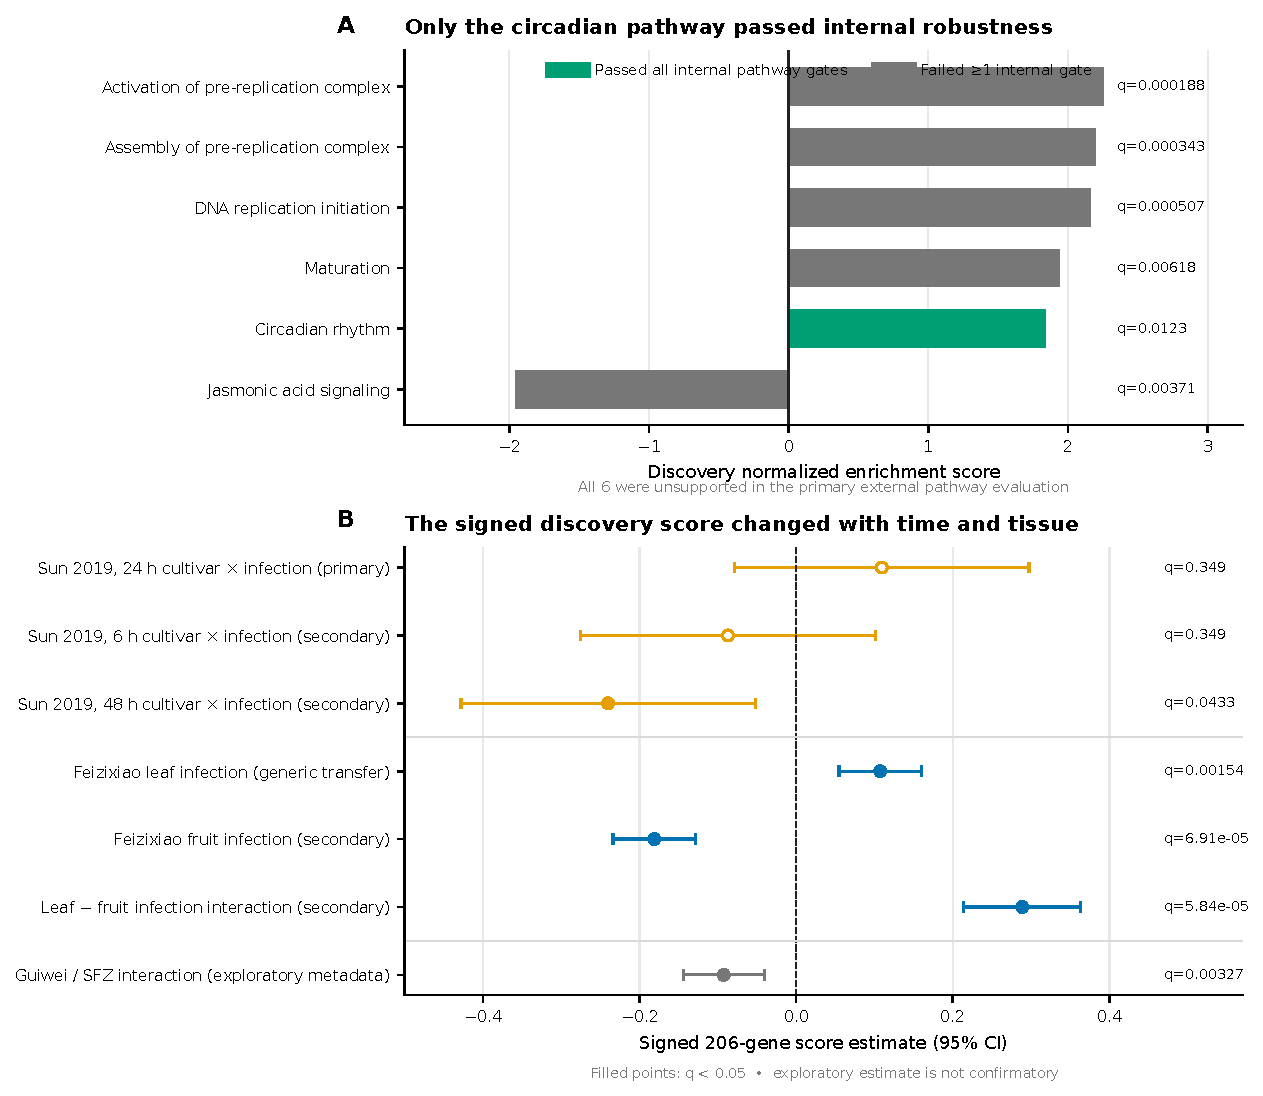
\includegraphics[width=0.92\textwidth]{figure4_pathways_signatures.pdf}
\caption{\textbf{Frozen pathway and signature evaluation.} (A) Discovery normalized enrichment scores for the six frozen pathways; only circadian rhythm passed all internal gates, and none was supported in the primary external evaluation. (B) The frozen signed 206-gene signature across the six non-exploratory external contrasts; filled points denote $\q<0.05$. The quarantined PRJNA1090613 estimate is in Figure~S3.}
\label{fig:pathways}
\end{figure}

\subsection{Conditional transcript-usage discovery remained internal}

Differential transcript usage was analyzed under a conditional gate registered in advance: stage-wise testing had to yield interpretable gene- and transcript-level error control, and no post hoc substitute was permitted if the gate failed. The gate passed, and 225 transcript-usage events across 152 genes were frozen from 15,790 tested transcripts (Figure~\ref{fig:dtu}A). External follow-up preserved the role separation of the cohorts (Figure~\ref{fig:dtu}B): in the primary cross-context study, 125 events were measurable but unsupported at the prespecified thresholds and 100 were not testable; in the generic-transfer study, annotation incompatibilities left all 225 untestable; and in the exploratory cohort, 4 events were supported and 5 contradictory; we report these outcomes descriptively and do not count them as primary external support, because that cohort's metadata could not be standardized. Transcript-level rewiring between cultivars therefore remains an internally supported, externally unconfirmed layer of the resource.

\begin{figure}[p]
\centering
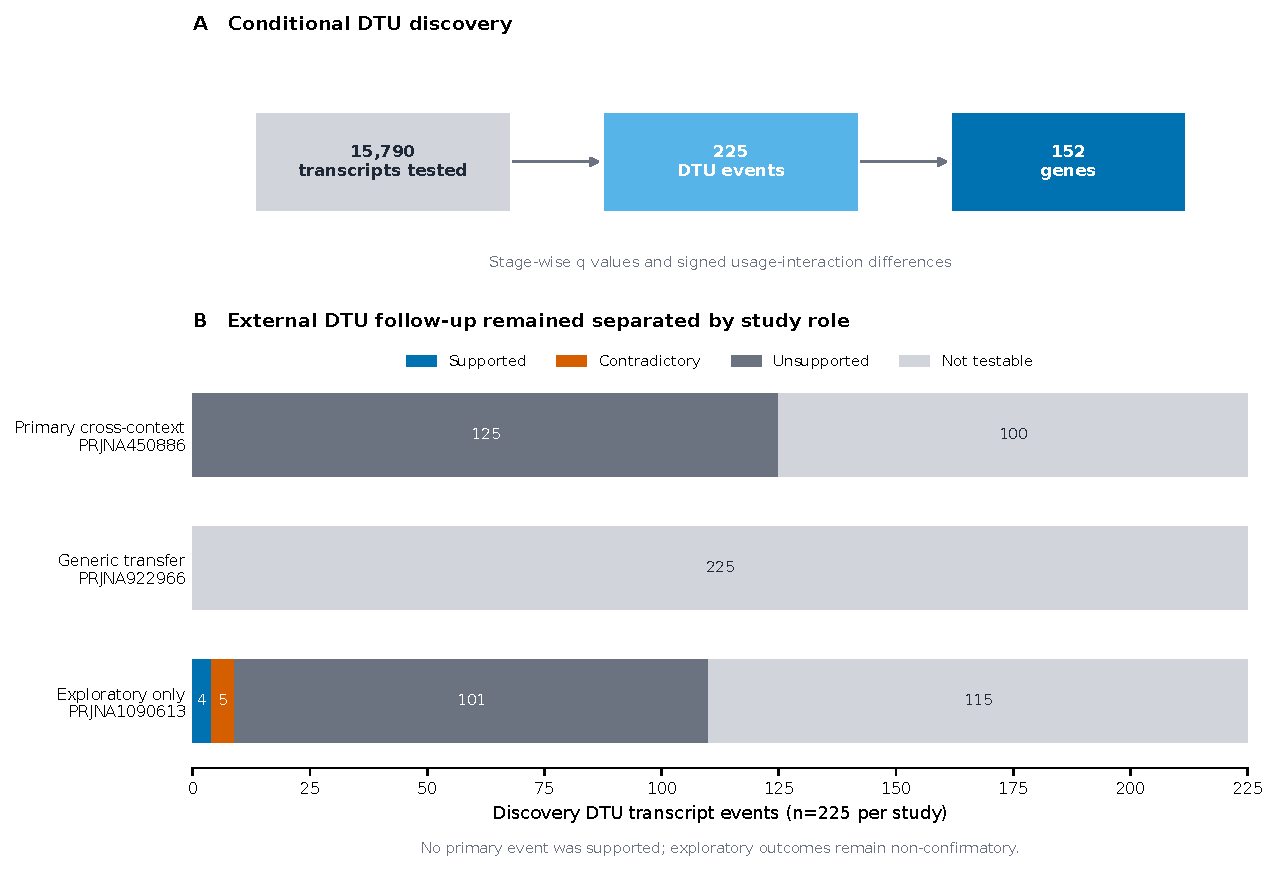
\includegraphics[width=0.98\textwidth]{figure5_transcript_usage.pdf}
\caption{\textbf{Conditional transcript usage.} (A) Discovery gate and event counts. (B) External follow-up of the 225 discovery events, separated by prespecified study role.}
\label{fig:dtu}
\end{figure}

\subsection{Orthogonal evidence: informative nulls and reference-ecosystem gaps}

The registered orthogonal evidence classes returned uniformly negative or non-testable results, and we report them as such rather than converting them into support. Computational annotation assigned family-level functional labels to 150 of the 206 candidates and left 56 unannotated, but no candidate met the registered high-confidence rule requiring two independent evidence classes with at least 70\% supported coverage and no architecture conflict, largely because precomputed InterPro domain architectures were unavailable for all 206 proteins in this non-model species (Figure~\ref{fig:ortho}A). Registered promoter-motif discovery tested 927 JASPAR plant position-weight matrices in strand-aware 1-kb and 2-kb windows against 100 expression- and GC-matched genomic background sets. No motif passed in more than 4 of 100 backgrounds against a required 80, and none passed FIMO sensitivity (Figure~\ref{fig:ortho}B). Small-RNA coherence was not testable because the frozen PmiREN reference contained no exact \textit{Litchi} entries.

A separate post hoc controlled comparison held the published 18-promoter totals, six explicitly reported exact-element strings plus one standard PlantCARE TCA-element variant, scoring rule, and multiplicity correction fixed while changing only the background (Supplementary S15). The 100,000-set randomized-GC rerun closely reproduced the exploratory result. Against 100 expression- and GC-matched genomic promoter sets, ARE lost significance, ABRE gained it, and MeJA-responsive, TCA, and TC-rich classes remained significant: four of seven classes passed under either strategy, but the identity of one class changed. Background construction therefore affected the result but did not by itself explain the exploratory/registered discrepancy. This comparison is provenance-limited: the archived exploratory package omitted the observed-motif input TSV, and exact recounting from the current canonical 18 promoters reproduced the published total only for ARE. Accordingly, it cannot rescue a functional regulatory claim or establish which foreground representation generated the other published totals. Published studies reusing any analyzed accession, including the primary external study itself [5], remain registered as prior interpretation rather than independent support.

\begin{figure}[p]
\centering
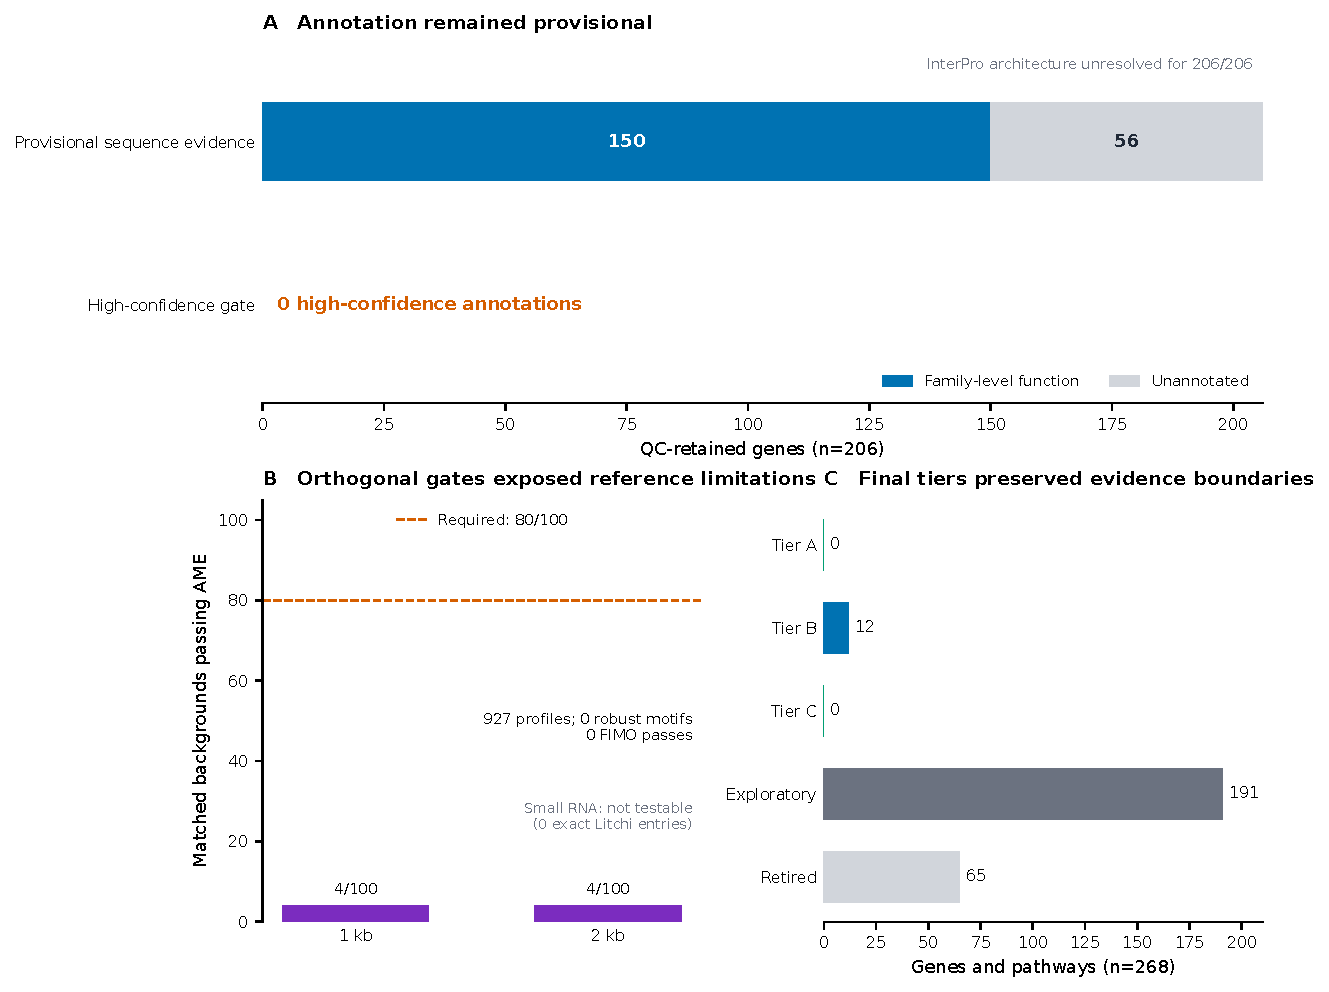
\includegraphics[width=0.98\textwidth]{figure6_orthogonal_tiers.pdf}
\caption{\textbf{Orthogonal evidence and final tiers.} (A) Annotation status of the 206 QC-retained genes. (B) Registered promoter-motif robustness and the small-RNA reference gate. (C) Deterministic final tiers over all 268 frozen entities.}
\label{fig:ortho}
\end{figure}

\subsection{Deterministic integration: an empty top tier, twelve Tier B genes, and visible retirements}

The registered tier rules integrate all evidence layers without discretion. Tier A required discovery, complete internal robustness, primary cross-context support, clean mapping and annotation, and at least one attributable orthogonal class; Tier B required discovery and full internal robustness with partial or non-testable external evidence; Tier C was reserved for a robust, externally supported pathway. Applied to the 268 frozen entities (262 statistical gene candidates and 6 pathways), the rules assigned no entity to Tier A or Tier C, 12 genes to Tier B, 191 entities to exploratory status, and 65 to retirement (Figure~\ref{fig:ortho}C). The retirements comprise the 56 statistical candidates removed by uniform mapping or gene-model control, the 5 genes contradicted for cross-context directional transport, and 4 candidates with candidate-level observed-mapping or annotation failures. These categories differ in kind, and the released tables preserve the distinction: mapping and annotation failures undermine the discovery itself, whereas an opposite direction in a different tissue and cultivar contrast may reflect genuine context specificity rather than an invalid discovery in the original context. Four internally robust genes, including a probable RPP8-like disease-resistance protein, were measurable but unsupported at the prespecified thresholds in the primary external evaluation and were therefore held at exploratory status rather than promoted. The two cross-context-supported genes likewise remain exploratory because they failed internal robustness. All contradictory and failed outcomes are released alongside the positive ones. We also note that Tier A was difficult to reach by construction in the current reference ecosystem: with the small-RNA class structurally untestable, no motif able to pass the family-wise rule, accession-linked literature excluded as independent support, and the two-class annotation rule unattainable without precomputed domain architectures, the orthogonal-class requirement could not realistically be satisfied by any gene. The empty top tier therefore reflects this structural constraint as much as the expression evidence itself.

The 12 Tier B genes are listed in Table~\ref{tab:tierb}. Nine were measurable in the primary external cohort, and all nine were direction-consistent with discovery, although none met the full support criteria. Figure~S1 exposes the normalized count of every individual discovery library for these 12 genes, the 2 cross-context-supported genes, and legacy highlights LITCHI001510 and LITCHI019519; every cultivar-treatment cell contains all three deposited replicates. Their annotations cluster around carbohydrate and cell-wall metabolism (a phosphomannomutase/phosphoglucomutase, a chloroplastic 1,4-alpha-glucan-branching enzyme, an ERD6-like sugar transporter, a serine carboxypeptidase), membrane transport (a WAT1-related protein), lipid signaling (a DIR1-like lipid-transfer protein, the \textit{Arabidopsis} ortholog of which is required for systemic acquired resistance), programmed-cell-death regulation (a BAG-family chaperone regulator), specialized metabolism (cytochrome P450 81Q32), RNA metabolism (ribonuclease J, exonuclease 1), chromatin-associated regulation (a homeobox-DDT protein), and one entirely unannotated gene.

\begin{table}[t]
\centering
\caption{\textbf{The twelve Tier B genes: internally robust genome-wide statistical candidates with direction-consistent but sub-threshold, or non-measurable, primary external evidence.} Discovery effects are interaction log2 fold changes (Yurong1 response minus Guiwei response); positive values indicate a stronger infection response in Yurong1. External columns give the primary 24-h pericarp estimate with 95\% confidence interval and family-adjusted \q; NM denotes genes not measurable in the external cohort.}
\label{tab:tierb}
\footnotesize
\setlength{\tabcolsep}{3pt}
\begin{tabular}{@{}llcccc@{}}
\toprule
\textbf{Gene} & \textbf{Family-level annotation} & \textbf{Disc.\ log2FC} & \textbf{Genome-wide \q} & \textbf{Ext.\ log2FC (95\% CI)} & \textbf{Ext.\ \q} \\
\midrule
LITCHI014613 & Sugar transporter ERD6-like 16 & $+3.69$ & $8.7\times10^{-6}$ & $+0.60$ ($-0.04$ to $+1.25$) & 0.27 \\
LITCHI015982 & WAT1-related protein & $+3.43$ & $7.8\times10^{-7}$ & $+0.77$ ($+0.07$ to $+1.48$) & 0.18 \\
LITCHI005805 & Phosphomannomutase/phosphoglucomutase & $+2.07$ & $5.5\times10^{-8}$ & NM & --- \\
LITCHI028926 & Exonuclease 1 & $+1.90$ & $5.7\times10^{-5}$ & $+0.32$ ($-0.63$ to $+1.28$) & 0.83 \\
LITCHI016077 & Serine carboxypeptidase 24 & $+1.81$ & $4.4\times10^{-5}$ & $+0.23$ ($-1.05$ to $+1.51$) & 0.89 \\
LITCHI013915 & 1,4-alpha-glucan-branching enzyme 3 & $+1.58$ & $4.4\times10^{-5}$ & $+0.53$ ($+0.10$ to $+0.95$) & 0.13 \\
LITCHI021546 & Homeobox-DDT domain protein RLT3 & $+1.31$ & $6.6\times10^{-5}$ & $+0.12$ ($-0.30$ to $+0.54$) & 0.83 \\
LITCHI022605 & Ribonuclease J & $+0.74$ & $2.9\times10^{-4}$ & $+0.14$ ($-0.34$ to $+0.62$) & 0.83 \\
LITCHI028717 & BAG-family chaperone regulator 4 & $-0.91$ & $1.8\times10^{-5}$ & $-1.20$ ($-2.52$ to $+0.12$) & 0.29 \\
LITCHI008721 & Unannotated protein & $-1.91$ & $7.9\times10^{-11}$ & NM & --- \\
LITCHI015740 & Putative lipid-transfer protein DIR1 & $-1.96$ & $1.2\times10^{-7}$ & $-0.21$ ($-1.10$ to $+0.69$) & 0.88 \\
LITCHI010877 & Cytochrome P450 81Q32 & $-2.77$ & $2.1\times10^{-7}$ & NM & --- \\
\bottomrule
\end{tabular}
\end{table}

\subsection{Parametric simulations quantify the interaction effects detectable with three libraries per cell}

The post hoc power analysis simulated negative-binomial counts from the fitted gene-wise means and dispersions while preserving the four-cell discovery design and the 24-h four-cell external design (Figure~S2; Supplementary S18). At each of 12 absolute interaction effects from 0 to 4 log2 units, 100 simulations were run sequentially. Genome-wide discovery used 19,445 tests with 262 injected targets per simulation, matching the observed statistical-candidate prevalence; the external analysis adjusted within the 177 frozen genes that passed the simulation's count and dispersion validity filters, with 2 injected targets matching the number of directionally supported genes. Seven additional genes were measurable in the observed 184-gene external contrast but were not fit-eligible for simulation, so the simulated multiplicity family is reported explicitly rather than equated with the observed family. The overall interpolated effect required for 80\% detection was 2.44 log2FC (5.4-fold) in discovery and 2.11 log2FC (4.3-fold) in the external candidate-family analysis. At a true $|$interaction log2FC$|$ of 1.5, overall detection probabilities were 62.7\% and 74.0\%, respectively. These values are conditional on fitted dispersions treated as known, deposited-library independence, and the simulated non-null prevalence; they quantify the low-power regime but cannot distinguish context dependence from absence of effect for any particular unsupported gene.

\section{Discussion}

The central finding of this unified analysis is methodological and biological at once: in the lychee--\Pl{} pathosystem, the genes that look most impressive in a single-cohort exploratory analysis and the genes that survive formal genome-wide inference are almost entirely different sets. The 18 exploratory candidates were chosen for large fold changes and defense-plausible annotations, yet none reached genome-wide significance for the cultivar-by-infection interaction, and two could not even be attributed unambiguously to a single locus. Conversely, the 16 genes that passed every internal robustness gate, and the 12 that reached Tier B, are dominated not by canonical pathogenesis-related families but by carbohydrate and cell-wall metabolism, transport, lipid signaling, and RNA metabolism, including one gene with no annotation at all. Neither observation would have been visible without running both stages, and together they quantify a selection effect that is likely to operate in any small-replicate transcriptomic study of this kind. One qualification applies throughout: the audit changed not only the statistical machinery but, for many of the 18 genes, the scientific question, from within-cultivar responsiveness to cultivar-dependent response, so the comparison measures survival under a stricter and partly different criterion rather than direct refutation of the original claims.

Why did the exploratory candidates fail the interaction audit? Three mechanisms, all anticipated by the reviewers of the exploratory report, are sufficient to explain the outcome. First, selection on observed fold change in a three-replicate contrast preferentially captures genes with high sampling variance, and their apparent effects regress when the full uncertainty is modeled: LITCHI019519's selected-gene contrast of $-3.4$ looked decisive, but its genome-wide interaction test carried a standard error of 1.14 and a \q-value of 0.106. Second, per-cultivar differential expression followed by informal comparison is not an interaction test; genes can differ dramatically in within-cultivar significance while their responses do not differ significantly between cultivars. Third, two candidates failed uniform-mappability control, a failure mode invisible to any analysis that trusts a single quantification path. None of this implies the exploratory candidates are biologically irrelevant; several retain large direction-consistent estimates and remain reasonable targets for quantitative PCR. Their evidentiary status, however, is now stated correctly: unconfirmed hypotheses, not validated markers.

The annotations of the genes that survive scrutiny suggest a recognizable, although still hypothetical, theme. Annotations related to cell-wall and sugar metabolism appear at every supported evidence level: among the Tier B genes, a phosphomannomutase/phosphoglucomutase, a starch-branching enzyme, an ERD6-like sugar transporter, and a serine carboxypeptidase; and among the two cross-context-supported genes, an alpha-xylosidase acting on xyloglucan. We emphasize that this is a qualitative clustering of family-level annotations over small gene sets, assembled from different genes at different evidence levels, and not a formal over-representation result; no enrichment test was performed, and several annotations are provisional. The pattern is nonetheless consistent with the emphasis on sugar metabolism and cell-wall reinforcement in prior comparisons of resistant and susceptible lychee cultivars [5], and with the general role of apoplastic sugar status and wall remodeling in oomycete resistance. The Tier B set also contains a DIR1-like lipid-transfer protein, whose \textit{Arabidopsis} counterpart is a mobile signal in systemic acquired resistance, and a BAG-family chaperone regulator; BAG proteins act as HSP70 co-chaperones within the chaperone networks that shape plant immune responses and immune-associated cell death [9]. The strong negative discovery enrichment of jasmonic acid signaling, although it did not survive external evaluation, is likewise a plausible axis of cultivar difference given the jasmonate-associated promoter elements suggested in the exploratory stage and the known antagonism between jasmonate and salicylate defense programs. We advance all of these as prioritized, testable hypotheses; the tier system exists precisely to prevent us from advancing them as more.

The external evaluation delivers a second structural lesson. The internally robust and externally supported sets did not overlap, but this disjunction carries almost no information on its own: with 16 and 2 genes selected from 206 candidates, the expected overlap under independence is 0.16 and zero overlap occurs with probability 0.85. The informative observations are continuous ones: discovery and external interaction effects were uncorrelated across the 184 measurable candidates, the frozen signature reversed sign between 24~h and 48~h in the external time course, and the same signature tracked infection in opposite directions in leaf and fruit of the transfer cohort. The straightforward reading is that the cultivar-dependent component of the early infection response is substantially tissue- and time-specific, so that a candidate's failure to transport from leaf at 24~h to pericarp at 48~h is expected behavior rather than evidence against the discovery. This has a practical corollary for breeding applications: expression-based resistance markers derived from one tissue and time point should not be assumed portable, and marker development for this pathosystem will require validation in the tissue and developmental window where deployment is intended.

The orthogonal layers contribute mainly disciplined null results, and we consider their inclusion one of the more useful aspects of the resource. The post hoc controlled PlantCARE comparison now isolates the background rule as far as the archived inputs permit. It shows that genomic expression/GC matching changes which class passes (ARE is replaced by ABRE) but does not eliminate the MeJA, TCA, or TC-rich signals when the published foreground totals are held fixed. Background choice is therefore not a sufficient explanation for the failure of the registered JASPAR analysis; the changed foreground, motif representation, scoring, and robustness rule remain consequential. Because the original observed-motif TSV was not archived and most published totals cannot be reproduced from the current canonical promoters, the controlled result is a provenance audit rather than evidence of regulatory function. The annotation and small-RNA outcomes likewise expose reference-ecosystem gaps (no precomputed InterPro architectures and no \textit{Litchi} entries in the frozen miRNA reference) that bound what any computational study of this species can currently claim.

Several limitations qualify all of the above. The deposited designs are small, with three libraries per cell, and the independence of those libraries at the level of source trees, pooling, and extraction is unreported, so our \q-values are conditional on deposited-library independence. The public metadata also leave the inoculation protocol underspecified, including the inoculum form (mycelia, sporangia, or zoospores), the developmental stage of the sampled leaves, and whether the tissue was wounded before inoculation, so all conclusions are additionally conditional on the depositors' experimental design. All quantification depends on a single reference assembly, and although uniform and observed mapping checks removed the clearest failure modes, residual reference bias cannot be excluded. The primary external cohort is deliberately heterogeneous with respect to the discovery cohort, which makes support conservative and non-support ambiguous; no genuinely independent replication cohort (same tissue, same time, different biological material) exists in the public record for this design. Unsupported external outcomes additionally conflate limited power, context dependence, and true absence of effect. The simulations quantify the first component: conditional 80\% minimum detectable effects were 2.44 log2FC (5.4-fold) for genome-wide discovery and 2.11 log2FC (4.3-fold) for candidate-family external evaluation, with still poorer performance among low-expression genes. These conditional curves do not identify which unsupported genes are context-specific or truly null. And the entire study is computational: no candidate, including the Tier B set, has been perturbed experimentally. The natural next steps are quantitative PCR of the Tier B genes in independently infected material of both discovery cultivars, functional tests of the alpha-xylosidase and DIR1-like candidates, and, for any regulatory hypothesis, direct assays such as promoter--reporter or chromatin-binding experiments rather than further motif counting.

\section{Conclusions}

By carrying a single pathosystem from exploratory candidate discovery through a prospectively registered genome-wide discovery framework with prespecified cross-context external evaluation, this study establishes which claims about cultivar-dependent responses of lychee to \Pl{} the current public data can and cannot support. It can support a set of 206 QC-retained genome-wide statistical interaction candidates, of which 19 are significant under both statistical frameworks, a stable core of 16 internally robust genes, 12 Tier B candidates whose annotations include cell-wall, sugar-metabolism, lipid-signaling, and RNA-metabolism functions, and 2 genes with cross-context support in an independent tissue and cultivar contrast. It cannot support the original 18 exploratory candidates as validated markers, any pathway- or signature-level claim of context-free transport, or any regulatory-element claim under matched-background testing. All frozen results, including nulls, contradictions, and retirements, are released with the analysis code and checksummed source data, so that the next stage of experimental validation can begin from an honest baseline.

\section{Materials and Methods}

\subsection{Study design, registration, and evidence vocabulary}

The confirmatory stage was governed by a time-stamped protocol, with amendments logged, distributed with the accompanying repository. The registration chronology is as follows. The exploratory stage was completed first, so the discovery dataset had already been analyzed, under different models, before registration. Protocol version 1.0.0 was frozen on 18 August 2026, with its SHA-256 hash (ef668486\ldots) recorded alongside the protocol text, before any confirmatory expression outcome was computed. The amendment log records 20 outcome-blind amendments (clarifications, implementation corrections, and optimizations, all time-stamped before any discovery or external expression outcome was viewed) and 3 post-outcome amendments confined to technical quality control and manifest verification, each marked as such. The primary external study had been published previously [5], and its headline biological conclusions were known to the analyst before registration; dataset roles and all thresholds were nevertheless fixed before any external count matrix was processed. Because all cohorts are public, the staged external unlock is a workflow-enforced computational safeguard, not blinding in the experimental sense. The protocol fixed dataset roles (Table~\ref{tab:roles}), statistical models, discovery and evaluation thresholds, conditional gates, empty-set behavior, and the vocabulary used throughout this paper: \emph{frozen} denotes a computed result fixed at a recorded checkpoint and never modified afterward; \emph{discovery} refers only to the registered genome-wide interaction analysis in PRJNA830488; \emph{robustness} refers only to predeclared sensitivity analyses within that cohort; \emph{cross-context support} denotes a passing frozen external test in a cohort that differs in tissue, comparator, or design, and is never described as replication; and \emph{orthogonal} evidence classes (annotation, motifs, small RNA, literature) are reported separately from expression support and cannot substitute for it. No external outcome could modify frozen discovery membership, signature weights, or thresholds.

\subsection{Exploratory-stage analyses (Stage 1)}

The exploratory stage analyzed the 12 GSE201243 libraries with FastQC v0.11.9 quality control, Trimmomatic v0.39 trimming, TopHat v2.0.12/Bowtie2 v2.2.3 alignment to the SCAU\_Lch\_v2.0 assembly (GCA\_019925255.1), HTSeq v2.0.2 union-mode counting, and DESeq2 v1.42.0 per-cultivar Wald contrasts (design $\sim$ treatment) with Benjamini--Hochberg adjustment at $P<0.05$ [10--15]. Candidate prioritization combined significance, fold-change magnitude, and annotation plausibility; structural, conserved-motif, and promoter analyses used TBtools-II v2.096, MEME v5.5.5, and PlantCARE [16--18]; and the promoter-background comparison tested observed \textit{cis}-element counts in the 18 candidate promoters against 100,000 randomized sets of eighteen 2-kb sequences with lychee-like GC content, scoring exact motifs and reverse complements, with one-sided empirical $P$-values adjusted by Benjamini--Hochberg [19]. The selected-gene interaction contrast was computed as log2FC(Yurong1, infected versus mock) $-$ log2FC(Guiwei, infected versus mock) over the prioritized genes and was explicitly labeled a prioritization effect size rather than a genome-wide test.

\subsection{Data provenance and eligibility}

National Center for Biotechnology Information and Gene Expression Omnibus metadata for all five cohorts were reconciled into a biological-unit registry (Supplementary S1). The original repository preserved accession decisions but not the historical query log, so search coverage was reconstructed retrospectively on 27 August 2026 and is not represented as prospective provenance. A broad NCBI GEO series query returned six records and a corresponding BioProject query returned seven; a narrow SRA cross-check returned 42 experiment-level records. After collapsing the GSE222652 super-series, excluding PRJNA1157370 because it used \textit{Colletotrichum gloeosporioides}, and excluding PRJNA268587/GSE63658 because it studied fruit senescence/storage without \Pl{} inoculation, the five prespecified cohorts remained (Supplementary S16a--b). Because source-tree, pooling, harvest, and extraction independence were not reported for the discovery libraries, all inferential \q-values are conditional on deposited-library independence. The primary model required at least three included libraries in every cultivar-treatment cell.

\subsection{Confirmatory preprocessing and quality gates}

Host (SCAU\_Lch\_v2.0) and pathogen references were combined with prefixed contig names to absorb pathogen-derived reads. Paired reads were checked with FastQC, trimmed with fastp [20], aligned with STAR two-pass mapping [21], counted at the gene level with featureCounts [22], and independently quantified with Salmon [23]. Libraries were excluded if fewer than 10 million read pairs survived trimming or fewer than 40\% of reads aligned uniquely; all 12 discovery libraries passed. GenMap-based exon-uniqueness scores [24] and candidate-level observed-mapping checks were fixed before discovery and used for the uniform mapping and observed mapping-sensitivity gates.

\subsection{Genome-wide discovery model}

DESeq2 [15] fitted gene counts with the design $\sim$ cultivar + treatment + cultivar:treatment (reference levels Guiwei, mock). The primary coefficient, cultivarYurong1:treatmentinfected, estimates the difference in infected-minus-mock response between Yurong1 and Guiwei. Genes required counts of at least 10 in at least three libraries; statistical candidates required genome-wide Benjamini--Hochberg $\q<0.05$ and $|\mathrm{log2FC}|\ge\log_2(1.5)$ [19]. The registered rule tests the point null of zero interaction and applies the effect threshold to the observed estimate. Post hoc sensitivity used DESeq2 with \texttt{lfcThreshold = log2(1.5)} and \texttt{altHypothesis = greaterAbs}, plus apeglm false-sign-or-small $s$-values for the same threshold; neither analysis modified frozen membership. To align the legacy audit with its original estimand, separate post hoc DESeq2 models ($\sim$ treatment) were fitted within Guiwei and Yurong1, using the same count matrix, 19,445-gene universe, and genome-wide Benjamini--Hochberg adjustment within each cultivar. Unshrunken maximum-likelihood estimates are reported throughout; apeglm-shrunken interaction estimates [25] were used only to define the signed signature weights over the 206 frozen genes. Mappability and gene-model metrics were computed for all 19,445 tested genes; as a sensitivity check, recomputing the Benjamini--Hochberg adjustment over only the 13,602 QC-eligible genes rediscovered all 206 frozen candidates plus 12 additional genes, confirming that applying quality control after significance testing was conservative here.

\subsection{Pathway and transcript-usage discovery}

Plant Reactome pathway memberships [26] were transported to lychee through one-to-one reciprocal-best DIAMOND protein matches to \textit{Oryza} [27], and pathway discovery applied the frozen genome-wide interaction statistic to this fixed mapping with camera, roast, and fgsea testing plus leading-edge-deletion and expression/length-matched null gates for robustness [28--30]. Differential transcript usage used Salmon transcript abundances analyzed with DRIMSeq and DEXSeq under stageR stage-wise error control [31--33]; the conditional inferential gate for interpretable two-level error control was registered in advance, and no substitute analysis was permitted had it failed.

\subsection{Internal robustness gates}

Each frozen gene was retested under Salmon-based gene-level quantification, edgeR quasi-likelihood interaction testing [34], a counts-per-million expression filter, and all leave-one-library-out refits, with predeclared criteria combined conjunctively; no additive scoring was used. The Salmon gate required direction agreement and an absolute effect difference of at most 0.5 log2 units; the edgeR analysis used the identical design matrix and interaction coefficient with TMM normalization, robust dispersion estimation (estimateDisp and glmQLFit with robust settings), and glmQLFTest, with Benjamini--Hochberg adjustment computed genome-wide over all 19,445 genes and a gate of genome-wide $\q<0.10$ plus direction agreement; the expression-filter gate refit the primary model after a counts-per-million filter; and the leave-one-library-out gate required direction agreement in all 12 refits and $\q<0.10$ in at least 10 of 12. The observed mapping-sensitivity gate removed candidates whose effect depended on ambiguously mapped reads. Frozen pathways required agreement across camera, roast, leading-edge deletion, and the matched-null comparison.

\subsection{External frozen evaluation}

PRJNA450886 was analyzed with the design $\sim$ cultivar $\times$ treatment $\times$ time, with time encoded as a categorical factor and 24~h as the reference level, so that the cultivar-by-treatment coefficient estimates the 24-h interaction and the three-way terms give the 6-h and 48-h contrasts; the primary estimand was the resistant-minus-susceptible cultivar-by-infection interaction at 24~h, with 6-h and 48-h contrasts secondary. Frozen candidate tests used Benjamini--Hochberg adjustment across the full candidate-by-contrast family, an absolute effect threshold of $\log_2(1.5)$, confidence intervals excluding zero, and discovery-direction agreement; opposite-direction passes were recorded as contradictory. PRJNA922966 was analyzed with $\sim$ tissue + treatment + tissue:treatment for generic-transfer tests, and PRJNA1090613 outcomes were confined to exploratory status by protocol. The frozen signed signature was evaluated as a library-level score with the same family-wise adjustment.

\subsection{Annotation, motif, small-RNA, and literature classes}

Representative proteins were chosen by longest coding sequence with lexicographic tie-breaking. Reviewed Swiss-Prot (release 2026\_02) DIAMOND matches [35], targeted InterPro/Pfam domain assignments [36], and one-to-one \textit{Oryza} orthology formed three separate annotation classes; the high-confidence label required at least two classes, at least 70\% supported coverage, and no architecture conflict. Promoter-motif analysis tested 927 JASPAR plant position-weight matrices [37] in strand-aware 1-kb and 2-kb promoter windows against 100 expression- and GC-matched background sets, with AME as the primary test, FIMO as sensitivity [38,39], robustness requiring passes in at least 80 of 100 backgrounds in both windows, and cognate transcription-factor expression required for attribution. The PmiREN bulk archive [40] was audited before small-RNA analysis; because it contained no exact \textit{Litchi} entries, the class was frozen as not testable and no study-derived reference was substituted. Published studies reusing any analyzed accession were registered as prior interpretation. For the post hoc controlled PlantCARE comparison, published observed totals across the 18 legacy promoters were fixed and tested against (i) 100,000 simulated sets of eighteen 2-kb sequences at 34\% GC and (ii) 100 genomic sets of eighteen promoters matched by mean-expression and promoter-GC quintiles with the same seeded minimum-distance rule used by the registered motif pipeline. The six reported motifs and one standard TCA variant, together with reverse complements, were counted and one-sided empirical $P$-values were adjusted across seven classes. The missing archived observed-motif TSV and canonical-promoter recount discrepancies were retained as explicit provenance limitations (Supplementary S15).

\subsection{Simulation-based power analysis}

Negative-binomial parametric simulations used DESeq2 maximum-a-posteriori gene dispersions and fitted sample means from the discovery counts and from the 24-h subset of PRJNA450886. Fitted cultivar and treatment main effects and size factors were retained, background-gene interaction coefficients were set to zero, and equal numbers of positive and negative effects were injected at 12 absolute log2FC values (0, 0.5, 0.75, 1, 1.25, 1.5, 1.75, 2, 2.5, 3, 3.5, 4). Each value had 100 simulations. Discovery injected 262 targets and applied Benjamini--Hochberg correction over 19,445 genes plus the registered effect filter. External simulation injected 2 targets among the 177 frozen genes passing the simulation count and dispersion validity filters and additionally required the prespecified sign and a 95\% interval excluding zero; the observed external table contained 184 measurable genes, seven of which were not fit-eligible for the simulation. Dispersions were treated as known during simulated Wald refits, making the curves conditional parametric power rather than a claim about population-level biological replication. Eighty-percent minimum detectable effects were linearly interpolated between grid points, with expression-quartile curves and Wilson intervals reported in Figure~S2.

\subsection{Tier rules, software versions, and reproducibility}

Tier A required discovery, complete internal robustness, primary cross-context support, clean mapping and annotation, and at least one attributable orthogonal class; Tier B required discovery and complete internal robustness with partial or non-testable primary external evidence; Tier C was reserved for a robust, externally supported pathway. Contradictory external direction or mapping/annotation failure retired an entity, and an empty Tier A was an allowed outcome. All stages ran under Snakemake 9.25.2 workflows [41] enforcing staged discovery, a controlled external unlock, verified cleanup, and SHA-256 manifests over inputs and outputs. Confirmatory executables were FastQC 0.12.1, fastp 1.3.6, STAR 2.7.10b, featureCounts/Subread 2.1.1, Salmon 2.5.1, MEME Suite/AME/FIMO 5.5.9, and DIAMOND 2.2.5; GenMap 1.3.0 is recoverable from the pinned specification although its executable is absent from the reconstructed environment. Statistical work used R 4.3.3/Bioconductor 3.18 with DESeq2 1.42.0, apeglm 1.24.0, edgeR 4.0.16, DRIMSeq 1.30.0, DEXSeq 1.48.0, stageR 1.24.0, and BiocParallel 1.36.0 (Supplementary S17 records the evidence status of every version). The resolved environment, synthetic fixtures, per-figure source data, and amendment log are distributed with the repository. All six main figures are regenerated from frozen result tables by a script that recomputes and asserts every headline count.

\section*{Declarations}

\textbf{Funding:} This work received no external funding. \textbf{Conflicts of interest:} The author declares no conflicts of interest. \textbf{Author contributions:} E.Z. conceived the study, performed all analyses, and wrote the manuscript.

\section*{Data and code availability}

All analyzed data are public: PRJNA830488 (GSE201243, discovery), PRJNA450886 (primary external), PRJNA922966 (GSE222651, generic transfer), PRJNA922965 (GSE222650, small RNA), and PRJNA1090613 (GSE262200, exploratory). The registered protocol, amendment log, complete result tables (all discovery statistics, robustness manifests, external tests, pathway/signature tests, transcript-usage results, annotation and orthogonal evidence, and the contradictory-results file), and the workflow code accompany this repository; a permanently archived release with a DOI, matching the submitted manuscript, will accompany the revised submission.

\section*{Supplementary information}

Supplementary tables S1--S18 provide the biological-unit registry, per-library quality control, all 19,445 discovery statistics (including composite-null and false-sign-or-small columns), robustness manifests, all external frozen tests, pathway/signature and transcript-usage results, annotation and orthology evidence, the small-RNA gate, all registered motif-background tests, the evidence registry, script/environment inventory, amendment log, within-cultivar legacy audit (S14), controlled PlantCARE background comparison (S15), reconstructed search queries and eligibility decisions (S16a--b), exact software versions (S17), and power minimum-detectable effects (S18). Figure~S1 shows replicate-level normalized counts, Figure~S2 the conditional power curves, and Figure~S3 the quarantined exploratory signature estimate. Every main and supplementary analytical figure has tab-separated source data where applicable.

\setcounter{figure}{0}
\renewcommand{\thefigure}{S\arabic{figure}}

\begin{figure}[p]
\centering
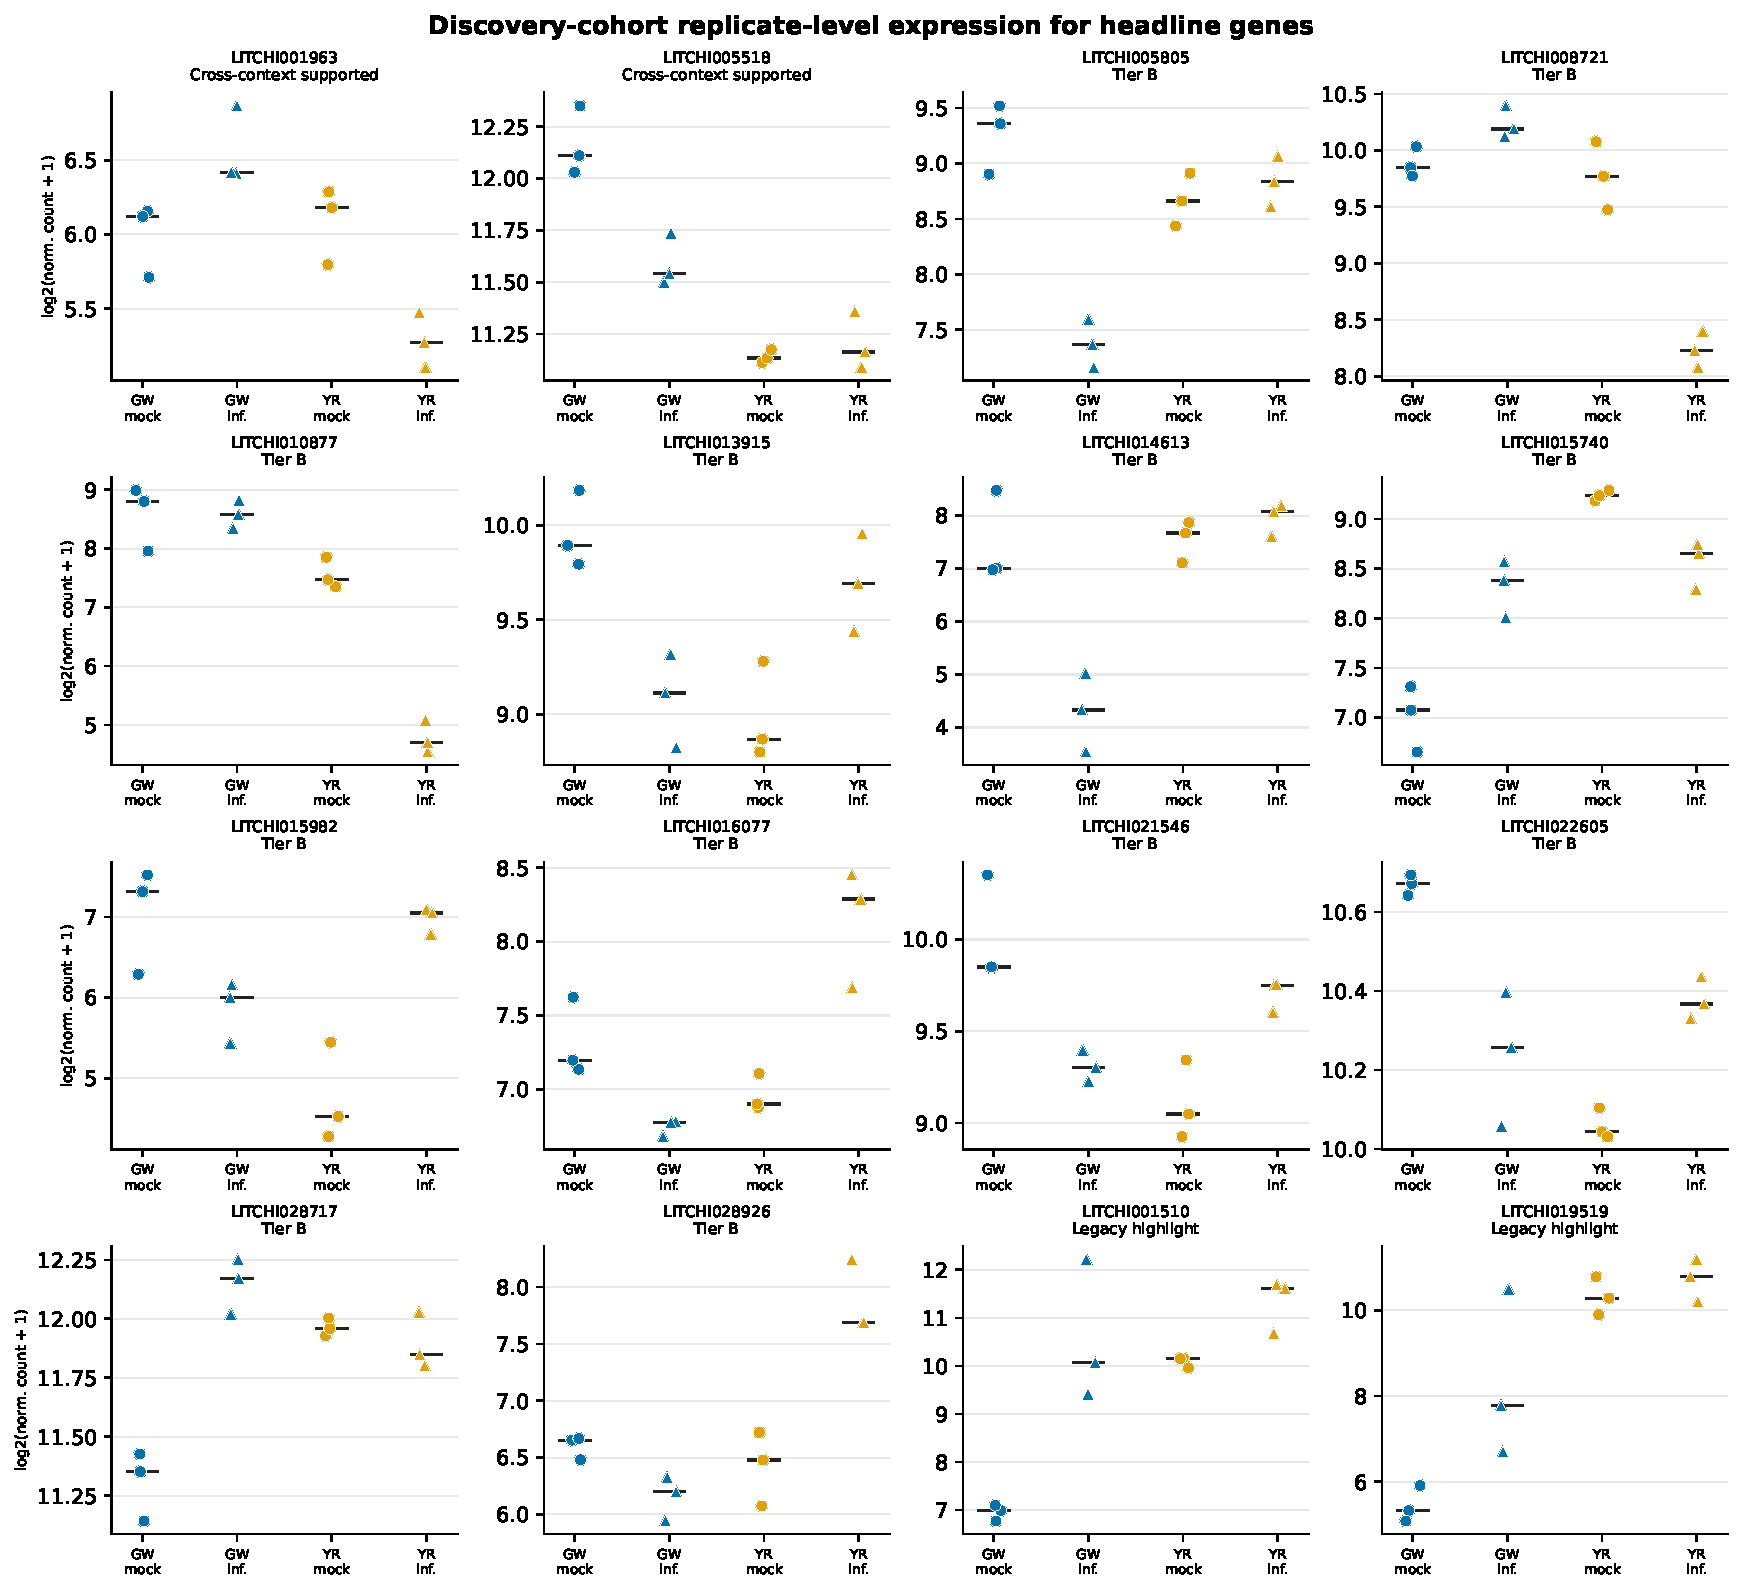
\includegraphics[width=0.98\textwidth]{FigureS1_replicate_level_counts.pdf}
\caption{\textbf{Replicate-level normalized counts for the two cross-context-supported genes, twelve Tier B genes, and two legacy highlights.} Points are individual deposited libraries; bars show cultivar-treatment medians.}
\label{fig:supp-counts}
\end{figure}

\begin{figure}[p]
\centering
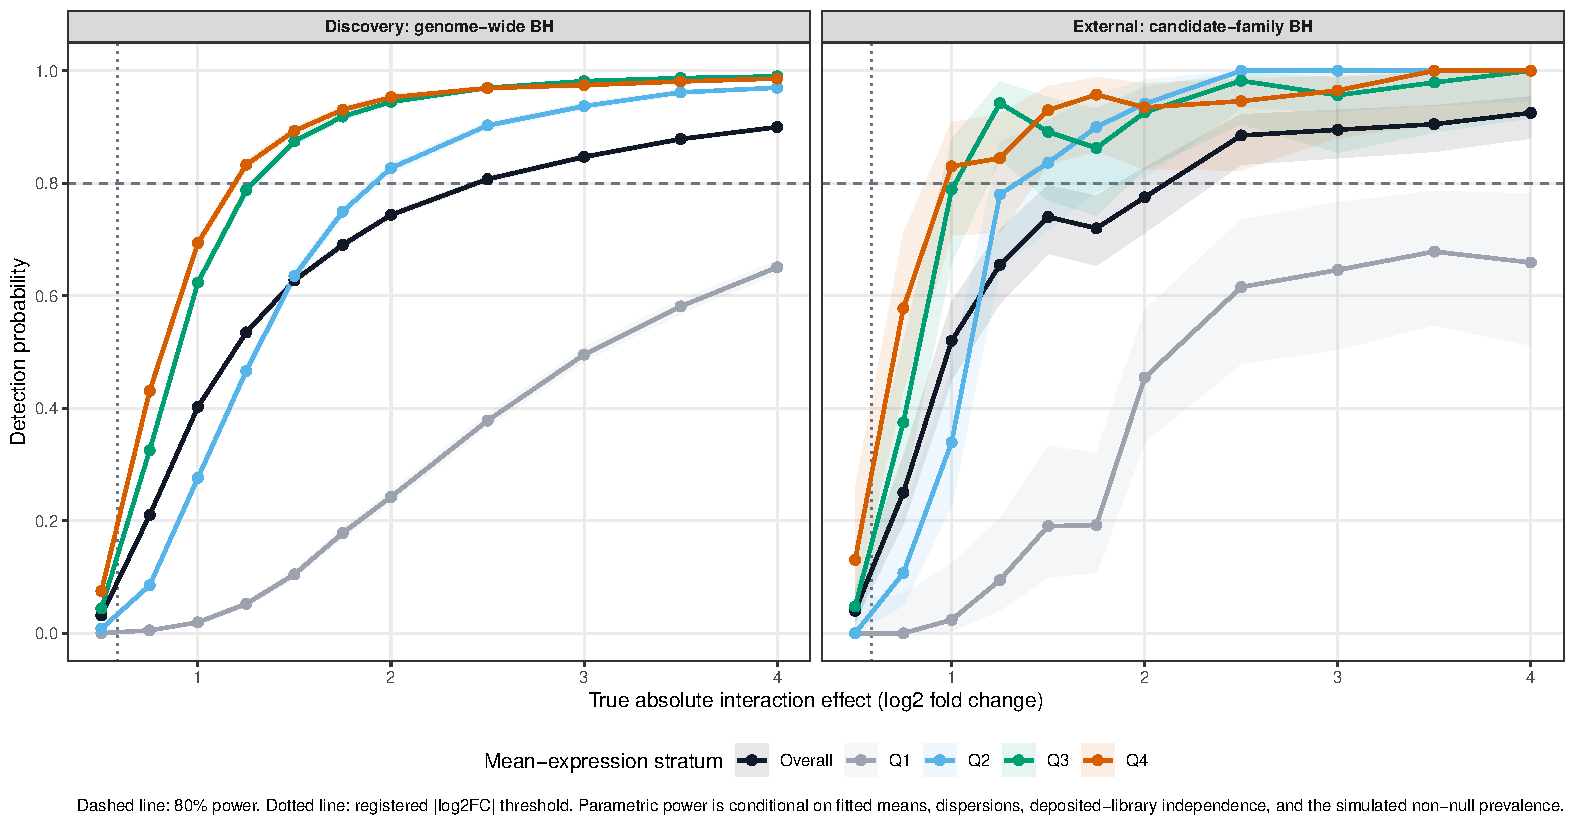
\includegraphics[width=0.9\textwidth]{FigureS2_power_analysis.pdf}
\caption{\textbf{Parametric detection probability for cultivar-by-infection effects under genome-wide discovery and candidate-family external adjustment.} Curves show the overall result and mean-expression quartiles; the dashed line marks 80\% power.}
\label{fig:supp-power}
\end{figure}

\begin{figure}[p]
\centering
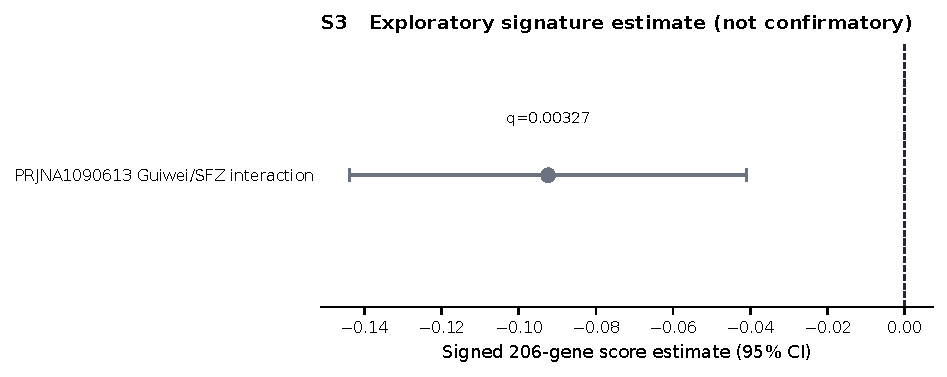
\includegraphics[width=0.7\textwidth]{figureS3_exploratory_signature.pdf}
\caption{\textbf{Quarantined PRJNA1090613 signed-signature estimate,} retained as exploratory rather than confirmatory evidence.}
\label{fig:supp-exploratory}
\end{figure}

\clearpage

\section*{References}
\begin{enumerate}[itemsep=1pt,leftmargin=1.6em]
\item Morton JF. Lychee. In: Fruits of Warm Climates. Winterville: Creative Resource Systems; 1987. p.~249--259.
\item Sun J, Gao Z, Zhang X, Zou X, Cao L, Wang J. Transcriptome analysis of \textit{Phytophthora litchii} reveals pathogenicity arsenals and confirms taxonomic status. PLoS ONE. 2017;12:e0178245.
\item Yi C, Jiang Y, Shi J, Qu H, Xue S, Duan X, et al. ATP-regulation of antioxidant properties and phenolics in litchi fruit during browning and pathogen infection process. Food Chemistry. 2010;118:42--47.
\item Hu G, Feng J, Xiang X, Wang J, Saloj\"arvi J, Liu C, et al. Two divergent haplotypes from a highly heterozygous lychee genome suggest independent domestication events for early and late-maturing cultivars. Nature Genetics. 2022;54:73--83.
\item Sun J, Cao L, Li H, Wang G, Wang S, Li F, et al. Early responses given distinct tactics to infection of \textit{Peronophythora litchii} in susceptible and resistant litchi cultivar. Scientific Reports. 2019;9:2810.
\item Liu H, Yan Q, Jiang Y, Shi F, Chen J, Cai C, et al. Identification of LcCDPKs and analysis of their expression patterns in response to downy mildew stresses in lychee. Journal of Fruit Science. 2023;40:442--456.
\item Li P, Li W, Zhou X, Situ J, Xie L, Xi P, et al. \textit{Peronophythora litchii} RXLR effector PlAvh202 destabilizes a host ethylene biosynthesis enzyme. Plant Physiology. 2023;193:756--774.
\item National Center for Biotechnology Information. GEO accession GSE201243. \url{https://www.ncbi.nlm.nih.gov/geo/query/acc.cgi?acc=GSE201243}.
\item Berka M, Kopeck\'a R, Berkov\'a V, Brzobohat\'y B, \v{C}ern\'y M. Regulation of heat shock proteins 70 and their role in plant immunity. Journal of Experimental Botany. 2022;73:1894--1909.
\item Andrews S. FastQC: a quality control tool for high throughput sequence data. Babraham Bioinformatics; 2010.
\item Bolger AM, Lohse M, Usadel B. Trimmomatic: a flexible trimmer for Illumina sequence data. Bioinformatics. 2014;30:2114--2120.
\item Kim D, Pertea G, Trapnell C, Pimentel H, Kelley R, Salzberg SL. TopHat2: accurate alignment of transcriptomes in the presence of insertions, deletions and gene fusions. Genome Biology. 2013;14:R36.
\item Anders S, Pyl PT, Huber W. HTSeq---a Python framework to work with high-throughput sequencing data. Bioinformatics. 2015;31:166--169.
\item Genome Warehouse. \textit{Litchi chinensis} SCAU\_Lch\_v2.0 assembly (GCA\_019925255.1). National Genomics Data Center, China National Center for Bioinformation.
\item Love MI, Huber W, Anders S. Moderated estimation of fold change and dispersion for RNA-seq data with DESeq2. Genome Biology. 2014;15:550.
\item Chen C, Chen H, Zhang Y, Thomas HR, Frank MH, He Y, et al. TBtools: an integrative toolkit developed for interactive analyses of big biological data. Molecular Plant. 2020;13:1194--1202.
\item Bailey TL, Elkan C. Fitting a mixture model by expectation maximization to discover motifs in biopolymers. In: Proceedings of the Second International Conference on Intelligent Systems for Molecular Biology. Menlo Park: AAAI Press; 1994. p.~28--36.
\item Lescot M, D\'ehais P, Thijs G, Marchal K, Moreau Y, Van de Peer Y, et al. PlantCARE, a database of plant cis-acting regulatory elements and a portal to tools for in silico analysis of promoter sequences. Nucleic Acids Research. 2002;30:325--327.
\item Benjamini Y, Hochberg Y. Controlling the false discovery rate: a practical and powerful approach to multiple testing. Journal of the Royal Statistical Society, Series B. 1995;57:289--300.
\item Chen S, Zhou Y, Chen Y, Gu J. fastp: an ultra-fast all-in-one FASTQ preprocessor. Bioinformatics. 2018;34:i884--i890.
\item Dobin A, Davis CA, Schlesinger F, Drenkow J, Zaleski C, Jha S, et al. STAR: ultrafast universal RNA-seq aligner. Bioinformatics. 2013;29:15--21.
\item Liao Y, Smyth GK, Shi W. featureCounts: an efficient general purpose program for assigning sequence reads to genomic features. Bioinformatics. 2014;30:923--930.
\item Patro R, Duggal G, Love MI, Irizarry RA, Kingsford C. Salmon provides fast and bias-aware quantification of transcript expression. Nature Methods. 2017;14:417--419.
\item Pockrandt C, Alzamel M, Iliopoulos CS, Reinert K. GenMap: ultra-fast computation of genome mappability. Bioinformatics. 2020;36:3687--3692.
\item Zhu A, Ibrahim JG, Love MI. Heavy-tailed prior distributions for sequence count data: removing the noise and preserving large differences. Bioinformatics. 2019;35:2084--2092.
\item Naithani S, Gupta P, Preece J, D'Eustachio P, Elser J, Garg P, et al. Plant Reactome knowledgebase: empowering plant pathway exploration and OMICS data analysis. Nucleic Acids Research. 2024;52:D1538--D1547.
\item Buchfink B, Xie C, Huson DH. Fast and sensitive protein alignment using DIAMOND. Nature Methods. 2015;12:59--60.
\item Wu D, Smyth GK. Camera: a competitive gene set test accounting for inter-gene correlation. Nucleic Acids Research. 2012;40:e133.
\item Wu D, Lim E, Vaillant F, Asselin-Labat ML, Visvader JE, Smyth GK. ROAST: rotation gene set tests for complex microarray experiments. Bioinformatics. 2010;26:2176--2182.
\item Korotkevich G, Sukhov V, Budin N, Shpak B, Artyomov MN, Sergushichev A. Fast gene set enrichment analysis. bioRxiv. 2021:060012.
\item Nowicka M, Robinson MD. DRIMSeq: a Dirichlet-multinomial framework for multivariate count outcomes in genomics. F1000Research. 2016;5:1356.
\item Anders S, Reyes A, Huber W. Detecting differential usage of exons from RNA-seq data. Genome Research. 2012;22:2008--2017.
\item Van den Berge K, Soneson C, Robinson MD, Clement L. stageR: a general stage-wise method for controlling the gene-level false discovery rate in differential expression and differential transcript usage. Genome Biology. 2017;18:151.
\item Robinson MD, McCarthy DJ, Smyth GK. edgeR: a Bioconductor package for differential expression analysis of digital gene expression data. Bioinformatics. 2010;26:139--140.
\item The UniProt Consortium. UniProt: the Universal Protein Knowledgebase in 2023. Nucleic Acids Research. 2023;51:D523--D531.
\item Jones P, Binns D, Chang HY, Fraser M, Li W, McAnulla C, et al. InterProScan 5: genome-scale protein function classification. Bioinformatics. 2014;30:1236--1240.
\item Rauluseviciute I, Riudavets-Puig R, Blanc-Mathieu R, Castro-Mondragon JA, Ferenc K, Kumar V, et al. JASPAR 2024: 20th anniversary of the open-access database of transcription factor binding profiles. Nucleic Acids Research. 2024;52:D174--D182.
\item McLeay RC, Bailey TL. Motif enrichment analysis: a unified framework and an evaluation on ChIP data. BMC Bioinformatics. 2010;11:165.
\item Grant CE, Bailey TL, Noble WS. FIMO: scanning for occurrences of a given motif. Bioinformatics. 2011;27:1017--1018.
\item Guo Z, Kuang Z, Wang Y, Zhao Y, Tao Y, Cheng C, et al. PmiREN: a comprehensive encyclopedia of plant miRNAs. Nucleic Acids Research. 2020;48:D1114--D1121.
\item M\"older F, Jablonski KP, Letcher B, Hall MB, Tomkins-Tinch CH, Sochat V, et al. Sustainable data analysis with Snakemake. F1000Research. 2021;10:33.
\end{enumerate}

\end{document}
